% arara: pdflatex
% arara: bibtex 
% arara: pdflatex 
% arara: pdflatex 
\documentclass[smallextended,natbib]{svjour3} %
\RequirePackage{fix-cm}
\usepackage[T1]{fontenc}
\usepackage[utf8]{inputenc}

%\usepackage{showframe}

\usepackage{textcomp} 
\usepackage{setspace}

\usepackage{caption} 
\usepackage{subcaption} 
\usepackage{afterpage} 

\usepackage{slantsc}
\usepackage{pifont}
\newcommand{\xmark}{\ding{54}}%
\newcommand{\ymark}{\ding{56}}%
\newcommand{\sunmark}{\ding{106}}%
\newcommand{\handmark}{\ding{43}}%

% \usepackage{lineno}
% \usepackage{pagecolor}
% \pagecolor{yellow!10!orange!5}

\usepackage[framemethod=tikz]{mdframed}
\mdfsetup{
skipabove=\baselineskip,
skipbelow=0\baselineskip,
innertopmargin=3pt,
innerbottommargin=3pt,
apptotikzsetting={\tikzset{mdfbackground/.append style={fill=red,fill opacity=0}}}
}



%% \usepackage{fontspec}
%% \newfontfamily{\tam}[Script=Tamil]{Lohit Tamil}
%% \defaultfontfeatures{Scale=MatchLowercase}

\usepackage{eurosym}

\usepackage{url}
%\usepackage{apacite}            % APA style citations
%\usepackage{apacdoc}

\let\oldcite\cite
\let\cite\citep
\let\citeA\oldcite
\let\citeNP\oldcite
\let\citeyear\citeyearpar
%\let\citeyear\cite

\usepackage{amsmath,amssymb}	% math structures and symbols
\usepackage{graphicx}		% including of graphics files in various formats
\usepackage{amsfonts}

\let\proof\relax
\let\endproof\relax 
\usepackage{amsthm}

\newtheorem*{ndef}{Definition of serendipity}

\newtheoremstyle{named}{.2\topsep}{}{\itshape}{}{\bfseries}{.}{}{}
\theoremstyle{named}


\usepackage{dialogue}
\usepackage{placeins}
\usepackage{tikz}
\usepackage{onimage}
\usetikzlibrary{positioning,backgrounds,fit,arrows,arrows.meta,shapes,shadows}
\usetikzlibrary{shapes.multipart}
\usepackage{wrapfig}
\usepackage{enumitem}
\usepackage{framed}

% \hypersetup{hidelinks}

\usepackage[xspace,mla]{ellipsis}

\definecolor{myyellow}{RGB}{242,226,149}
\definecolor{mygreen}{RGB}{144,238,144}
\definecolor{mypink}{RGB}{255,182,193}
\definecolor{myorange}{RGB}{255,165,0}
\definecolor{myblue}{RGB}{0,204,204}

\usepackage{xparse}
\NewDocumentCommand\StickyNote{O{4cm}mmO{4cm}}{%
\begin{tikzpicture}
\node[
drop shadow={
  shadow xshift=2pt,
  shadow yshift=-4pt
},
inner xsep=7pt,
fill=#2,
xslant=-0.05,
yslant=0.05,
inner ysep=10pt
] {\parbox[t][#1][c]{#4}{#3}};
\end{tikzpicture}%
}

%\urldef{\mailsa}\path|{j.corneli,s.colton}@gold.ac.uk|
%\urldef{\mailsb}\path|a.pease@dundee.co.uk|

%% \newcommand{\keywords}[1]{\par\addvspace\baselineskip
%% \noindent\keywordname\enspace\ignorespaces#1}

\usepackage{array,booktabs}
\newcommand{\tcap}[1]{
\begin{minipage}{.7in}
{\centering #1 \par}
\end{minipage}
}

\newcommand{\inlineitem}[1]{%
\begingroup%
\setlength\itemindent{-1em}%
\item[]%
\begin{minipage}{.96\textwidth}%
#1%
\end{minipage}%
\endgroup
}


\usepackage[ocgcolorlinks,citecolor=blue]{hyperref}

% Patch for just citing years are cited
\usepackage{etoolbox}

\makeatletter

% Patch case where name and year are separated by aysep
\patchcmd{\NAT@citex}
  {\@citea\NAT@hyper@{%
     \NAT@nmfmt{\NAT@nm}%
     \hyper@natlinkbreak{\NAT@aysep\NAT@spacechar}{\@citeb\@extra@b@citeb}%
     \NAT@date}}
  {\@citea\NAT@nmfmt{\NAT@nm}%
   \NAT@aysep\NAT@spacechar\NAT@hyper@{\NAT@date}}{}{}

% Patch case where name and year are separated by opening bracket
\patchcmd{\NAT@citex}
  {\@citea\NAT@hyper@{%
     \NAT@nmfmt{\NAT@nm}%
     \hyper@natlinkbreak{\NAT@spacechar\NAT@@open\if*#1*\else#1\NAT@spacechar\fi}%
       {\@citeb\@extra@b@citeb}%
     \NAT@date}}
  {\@citea\NAT@nmfmt{\NAT@nm}%
   \NAT@spacechar\NAT@@open\if*#1*\else#1\NAT@spacechar\fi\NAT@hyper@{\NAT@date}}
  {}{}

\makeatother


% color for links

\makeatletter
\AtBeginDocument{%
    \newlength{\temp@x}%
    \newlength{\temp@y}%
    \newlength{\temp@w}%
    \newlength{\temp@h}%
    \def\my@coords#1#2#3#4{%
      \setlength{\temp@x}{#1}%
      \setlength{\temp@y}{#2}%
      \setlength{\temp@w}{#3}%
      \setlength{\temp@h}{#4}%
      \adjustlengths{}%
      \my@pdfliteral{\strip@pt\temp@x\space\strip@pt\temp@y\space\strip@pt\temp@w\space\strip@pt\temp@h\space re}}%
    \ifpdf
      \typeout{In PDF mode}%
      \def\my@pdfliteral#1{\pdfliteral page{#1}}% I don't know why % this command...
      \def\adjustlengths{}%
    \fi
    \ifxetex
      \def\my@pdfliteral #1{\special{pdf: literal direct #1}}% isn't equivalent to this one
      \def\adjustlengths{\setlength{\temp@h}{-\temp@h}\addtolength{\temp@y}{1in}\addtolength{\temp@x}{-1in}}%
    \fi%
    \def\Hy@colorlink#1{%
      \begingroup
        \ifHy@ocgcolorlinks
          \def\Hy@ocgcolor{#1}%
          \my@pdfliteral{q}%
          \my@pdfliteral{7 Tr}% Set text mode to clipping-only
        \else
          \HyColor@UseColor#1%
        \fi
    }%
    \def\Hy@endcolorlink{%
      \ifHy@ocgcolorlinks%
        \my@pdfliteral{/OC/OCPrint BDC}%
        \my@coords{0pt}{0pt}{\pdfpagewidth}{\pdfpageheight}%
        \my@pdfliteral{F}% Fill clipping path (the url's text) with
                           % current color
        %
        \my@pdfliteral{EMC/OC/OCView BDC}%
        \begingroup%
          \expandafter\HyColor@UseColor\Hy@ocgcolor%
          \my@coords{0pt}{0pt}{\pdfpagewidth}{\pdfpageheight}%
          \my@pdfliteral{F}% Fill clipping path (the url's text)
                             % with \Hy@ocgcolor
        \endgroup%
        \my@pdfliteral{EMC}%
        \my@pdfliteral{0 Tr}% Reset text to normal mode
        \my@pdfliteral{Q}%
      \fi
      \endgroup
    }%
}
\makeatother

\begin{document}

% TITLE INFORMATION
\title{Modelling serendipity in a computational context\thanks{This research was supported by the Engineering and Physical Sciences Research Council through grants EP/L00206X, EP/J004049 as well as EP/L015846/1 and the Future and Emerging Technologies (FET) programme within the Seventh Framework Programme for Research of the European Commission, under FET-Open Grant numbers: 611553 (COINVENT) and 611560 (WHIM).}}
\author{Joseph Corneli \and Christian Guckelsberger \and Anna Jordanous \and Alison Pease \and Simon Colton}
\institute{Department of Computing, Goldsmiths College, University of London\\
\and
School of Computing, University of Dundee
\and
School of Computing, University of Kent}
\date{\today}

\titlerunning{Modelling serendipity in a computational context}
\authorrunning{~}

\maketitle

\begin{abstract}
%
Most prior work that deals with serendipity in a computing context only considers the role it plays in ``discovery'', but we argue that serendipity also includes an important ``invention'' aspect.
% \section{Literature review} \label{sec:literature-review}

In this section, we give a short overview covering the etymology of
the term ``serendipity'' and trace its development in order to pin
down the key commonalities from many definitions and instances.  In
particular, we point out key conditions of serendipity, their
components and general characteristics, including environmental
factors.  The structure of this section follows and updates an earlier
survey from \citeA{pease2013discussion}, drawing connections with our
formal model described above.

\subsection{Etymology and selected definitions} \label{sec:overview-serendipity}
The English term ``serendipity'' derives from the 1302 long poem \emph{Eight Paradises}, written in Persian by the Sufi poet Am\={\i}r Khusrow in Uttar Pradesh.\footnote{\url{http://en.wikipedia.org/wiki/Hasht-Bihisht}}  In the English-speaking world, its first chapter became known as ``The Three Princes of Serendip'', where ``Serendip'' represents the Old Tamil-Malayalam word for Sri Lanka (%{\tam சேரன்தீவு},
\emph{Cerantivu}), ``island of the Ceran kings.''

The term ``serendipity'' is first found in a 1757 letter by Horace Walpole to Horace Mann:
\begin{quote}
\emph{``This discovery is almost of that kind which I call serendipity, a very expressive
word} \ldots \emph{You will understand it better by the derivation than by the
definition. I once read a silly fairy tale, called The Three Princes of Serendip:
as their Highness travelled, they were always making discoveries, by accidents
\& sagacity, of things which they were not in quest of}[.]''~\cite[p. 633]{van1994anatomy}
\end{quote}
The term became more widely known in the 1940s through studies of serendipity as a factor in scientific discovery, surveyed by Robert Merton and Elinor Barben \citeyear{merton} in their 1957 analyis ``The Travels and Adventures of Serendipity, A Study in Historical Semantics and the Sociology of Sciences''.  Merton and Barben define the term as follows:
\begin{quote}
\emph{``The serendipity pattern refers to the fairly common experience of observing
an unanticipated, anomalous and strategic datum which becomes the occasion
for developing a new theory or for extending an existing theory.''} \cite[p. 635]{van1994anatomy}
\end{quote}
In 1986, Philippe Qu\'eau described serendipity as ``the art of
finding what we are not looking for by looking for what we are not
finding'' \cite{eloge-de-la-simulation}, as quoted in
\cite[p. 121]{Campos2002}.  Pek van Andel
\citeyear[p. 631]{van1994anatomy} describes it simply as ``the art of
making an unsought finding''.


Roberts \citeyear[pp. 246--249]{roberts} records 30 entries for the term ``serendipity'' from English language dictionaries dating from 1909 to 1989.  
%
Classic definitions require the investigator not to be aware of the problem they serendipitously solve, but this criterion has largely dropped from dictionary definitions. Only 5 of Roberts' collected definitions explicitly say ``not sought for.''  Roberts characterises ``sought findings'' in which an accident leads to a discovery with the term \emph{pseudoserendipity} \cite{chumaceiro1995serendipity}.
%
While Walpole initially described serendipity as an event, it has
since been reconceptualised as a psychological attribute, a matter of
sagacity on the part of the discoverer: a ``gift'' or ``faculty'' more
than a ``state of mind.''  Only one of the collected definitions, from
1952, defined it solely as an event, while five define it as both
event and attribute.

However, there are numerous examples that exhibit features of
serendipity which develop on a social scale rather than an individual
scale.  For instance, between Spencer Silver's creation of high-tack,
low-adhesion glue in 1968, the invention of a sticky bookmark in 1973,
and the eventual launch of the distinctive canary yellow re-stickable
notes in 1980, there were many opportunities for
Post-its\texttrademark\ \emph{not} to have come to be
\cite{tce-postits}. Accordingly, Merton and Barber argue that the
psychological perspective needs to be integrated with a
\emph{sociological} one.\footnote{ ``For if chance favours prepared
  minds, it particularly favours those at work in microenvironments
  that make for unanticipated sociocognitive interactions between
  those prepared minds. These may be described as serendipitous
  sociocognitive microenvironments'' \cite[p. 259--260]{merton}.}
Large-scale scientific and technical projects generally rely on the
``convergence of interests of several key actors''
\cite{companions-in-geography}, along with other supporting cultural
factors.  Umberto Eco \citeyear{eco2013serendipities} focuses on the
historical role of serendipitous mistakes and falsehoods in the
production of knowledge.

It is important to note that serendipity is usually discussed within
the context of \emph{discovery}, rather than \emph{creativity},
although in typical parlance these terms are closely related
\cite{jordanous12jims}.  In our definition of serendipity, we have
made use of Henri Bergson's distinction:
\begin{quote}
``\emph{Discovery, or uncovering, has to do with what already exists,
    actually or virtually; it was therefore certain to happen sooner
    or later.  Invention gives being to what did not exist; it might
    never have happened.}''~\cite{bergson2010creative}
\end{quote}
As we have indicated serendipity would seem to require features of
both; that is, the discovery of something unexpected and the invention
of an application for the same.  We must complement \emph{analysis}
with \emph{synthesis} \cite{delanda1993virtual}.  The balance between
these two features will differ from case to case.

In the next subsection we will review several historical examples.
First, one further point should be made with reference to the ``The
Three Princes of Serendip''.  Prior to Walpole's coinage, this story
had been adapted by Voltaire into an early chapter of \emph{Zadig},
and in turn ``the method of Zadig'' informed subsequent approaches
both to fiction writing and natural science.  This method is rooted
firstly in discovery:

\begin{quote}
``[Zadig] \emph{pry’d into the Nature and Properties of Animals and
    Plants, and soon, by his strict and repeated Enquiries, he was
    capable of discerning a Thousand Variations in visible Objects,
    that others, less curious, imagin’d were all
    alike.}''~\cite[pp. 21--22]{zadig}
\end{quote}

\noindent Secondly, from disparate observations, Zadig is often able
to assemble a coherent picture:
\begin{quote}
\emph{It was his peculiar Talent to render Truth as obvious as
  possible: Whereas most Men study to render it intricate and
  obscure.}~\cite[p. 54]{zadig}
\end{quote}
Similarly, but in reverse, a coherent picture may be reduced to
fragmented pieces each of which may tell a very different story from
the whole.  This is illustrated in Zadig's misadventure with a broken
tablet, in which one fragment of a poem of praise reads as treasonous
provocation.  In describing the various features of serendipity below,
we will draw connections with the schematic diagram presented in
Section \ref{specs-overview}, in order to unfold the multifaceted
notion of serendipity.

\subsection{Connections between prior literature on serendipity and our formal definition} \label{sec:connections-to-formal-definition}

\subsubsection*{Key condition for serendipity}

\begin{itemize}
\item \textbf{Focus shift}: ``\emph{After removing several of the
  burdock burrs (seeds) that kept sticking to his clothes and his
  dog's fur,}~[de Mestral]~\emph{became curious as to how it
  worked. He examined them under a microscope, and noted hundreds of
  `hooks' that caught on anything with a loop, such as clothing,
  animal fur, or hair. He saw the possibility of binding two materials
  reversibly in a simple fashion, if he could figure out how to
  duplicate the hooks and loops.}''~\cite{wiki:velcro}
%
\inlineitem{This corresponds to the identification of $T^\star$, which
  is common to both sides of the diagram.  \citeA{creativity-crisis}
  write that: ``To be creative requires divergent thinking (generating
  many unique ideas) and then convergent thinking (combining those
  ideas into the best result).''  Accordingly $T^\star$ may be thought
  of as an evolving vector of interesting possibilities or ``strategic data'' \cite[p. 507]{merton1948bearing}.  In de
  Mestral's case, the initial idea of a hook-and-loop fastener
  occurred in 1941 -- followed by a full decade of experimentation
  before he was ready to file a patent claim.  }
\end{itemize}

\subsubsection*{Components of serendipity}

\begin{itemize}
\item \textbf{Prepared mind}: 
Fleming's ``prepared mind'' included his focus
on carrying out experiments to investigate influenza as well as his
previous experience that foreign substances in petri dishes can kill
bacteria.  He was concerned above all with the question ``Is there a
substance which is harmful to harmful bacteria but harmless to human
tissue?''  \cite[p. 161]{roberts}.
%%
%
\inlineitem{This corresponds to the prior
  training $p$ and $p^{\prime}$ in our diagram.}
\item \textbf{Serendipity trigger}: The trigger does not directly
  cause the outcome, but rather, inspires a new insight.  It was long
  known by Quechua medics that cinchona bark stops shivering.  In
  particular, it worked well to stop shivering in malaria patients, as
  was observed when malarial Europeans first arrived in Peru.  The
  joint appearance of shivering Europeans and a South American remedy
  was the trigger.  That an extract from cinchona bark can cure and
  can even prevent malaria was subsequently revealed.
%
\inlineitem{This corresponds to the stimulus $T$ in our diagram.}
%%
\item \textbf{Bridge}: These include reasoning techniques, such as
  abductive inference (what might cause a clear patch in a petri
  dish?); analogical reasoning (de Mestral constructed a target domain
  from the source domain of burs hooked onto fabric); and conceptual
  blending (Kekul\'e blended his knowledge of molecule structure with
  his vision of a snake biting its tail).  The bridge may also rely on
  new social arrangements, such as the formation of cross-cultural
  research networks.
%
\inlineitem{This corresponds to the actions based on $p^{\prime}$
  taken on $T^\star$ leading to $R$.}
%%
\item \textbf{Result}: This may be a new product, artefact, process,
  hypothesis, a new use for a material substance, and so on.  The
  outcome may contribute evidence in support of a known hypothesis, or
  a solution to a known problem.  Alternatively, the result may itself
  be a {\em new} hypothesis or problem.  The result may be a
  ``pseudoserendipitous'' in the sense that it was {\em sought}, while
  nevertheless arising from an unknown, unlikely, coincidental or
  unexpected source.  More classically, it is an \emph{unsought}
  finding, such as the discovery of the Rosetta stone.
%
\inlineitem{This corresponds to our $R$.  Note that $R$ may imply
  updates to $p$ or $p^{\prime}$ in further phases of research.}
\end{itemize}

\subsubsection*{Dimensions of serendipity}

Whereas the foregoing items are the central features of the
definition, the following further characterise the circumstances under
which serendipity occurs in practice.

\begin{itemize}
\item \textbf{Chance}: Fleming \citeyear{fleming} noted: ``There are
  thousands of different moulds'' -- and ``that chance put the mould
  in the right spot at the right time was like winning the Irish
  sweep.''
%
\inlineitem{One must assume that relatively few triggers $T^\star$
  that are identified as interesting actually lead to useful results;
  in other words, the process is fallible.}
%%
\item \textbf{Curiosity}: Venkatesh Rao \citeyear{rao2011tempo} refers
  to a \emph{cheap trick} that takes place early on in a narrative in
  order to establish the preliminary conditions of order.  Curiosity
  with can play this role, and can dispose a creative person to begin,
  or to continue, a search into unfamiliar territory.
%
\inlineitem{The prior training $p$ causes interesting features to be
  extracted, even if they are not necessarily useful; $p^{\prime}$
  asks how these features \emph{might} be useful.  }
%%
\item \textbf{Sagacity}: This old-fashioned word is related to
  ``wisdom,'' ``insight,'' and especially to ``taste'' -- and
  describes the attributes, or skill, of the discoverer that
  contribute to forming the bridge between the trigger and the result.
  In many cases, such as an entanglement with cockle-burs, many others
  will have already been in a similar position and not obtained an
  interesting result.  Once a phenomenon has been identified as
  interesting, the disposition of the investigator may lead to a
  dogged pursuit of a useful application or improvement.
%
\inlineitem{Rather than a simple look-up
  rule, $p^{\prime}$ involves creating new knowledge.}
%%
\item \textbf{Value}: Note that the chance ``discovery'' of, say, a
  \pounds 10 note may be seen as happy by the person who finds it,
  whereas the loss of the same note would generally be regarded as
  unhappy.  Positive judgements of serendipity by a third party would
  be less likely in scenarios in which ``One man's loss is another
  man's gain'' than in scenarios where ``One man's trash is another
  man's treasure.''  If possible we prefer this sort of independent
  judgement \cite{jordanous:12}.
%
\inlineitem{The evaluation $|R|>0$ may be carried out ``locally'' (as
  an embedded part of the process of invention of $R$) or ``globally''
  (i.e.~as an external process).  }
\end{itemize}

\subsubsection*{Environmental factors}

\begin{itemize}
\item \textbf{Dynamic world}: Information about the world develops
  over time, and is not presented as a complete, consistent whole.  In
  particular, value may come later.  Van Andel
  \citeyear[p. 643]{van1994anatomy} estimates that in twenty percent
  of innovations ``something was discovered before there was a demand
  for it.''
%
\inlineitem{$T$ (and $T^\star$) appears within a stream of data with
  indeterminacy.  There is a further feedback loop, insofar as
  products $R$ influence the future state.}
%%
\item \textbf{Multiple contexts}: One of the dynamical aspects at play
  may be the discoverer going back and forth between different
  contexts, with different stimuli.  3M employee Arthur Fry sang in a
  church choir and needed a good way to mark pages in his hymn book;
  he happened to have been attending seminars offered by his colleague
  Silver about restickable glue.
%
\inlineitem{This is reflected directly in our model by the difference
  between the ``context of discovery'' involving prior preparations
  $p$, and the ``context of invention'' involving prior preparations
  $p^{\prime}$.  Both of these may be subdivided further.}
%%
\item \textbf{Multiple tasks}: Even within what would typically be
  seen as a single context, a discoverer may take on multiple tasks
  that segment the context into sub-contexts, or that cause the
  investigator to look in more than one direction.  The tasks may have
  an interesting \emph{overlap}, or they may point to a \emph{gap} in
  knowledge.  As an example of the latter, Penzias and Wilson used a
  large antenna to detect radio waves that were relayed by bouncing
  off of satellites.  After they had removed interference effects due
  to radar, radio, and heat, they found residual ambient noise that
  couldn't be eliminated \cite{wiki:cosmic-radiation}.
%
\inlineitem{Both $T$ and $T^\star$ may be multiple, causing an
  individual process to fork into communicating sub-processes that
  involve different skills sets.}
%%
\item \textbf{Multiple influences}: The ``bridge'' from trigger to
  result is often found through a social network, thus, for instance
  Penzias and Wilson only understood the significance of their work
  after reading a preprint by Jim Peebles that hypothesised the
  possibility of measuring radiation released by the big bang
  \cite{wiki:cosmic-radiation}.
%
\inlineitem{The process as a whole may be multiplied out among
  different communicating investigators.}
\end{itemize}

We survey literature describing serendipitous discovery+invention in science and technology.
% \section{Serendipity in a computational context} \label{sec:computational-serendipity}

The 13 criteria from Section \ref{sec:literature-review}
specify the conditions and preconditions that are conducive to
serendipitous discovery.  Here, we revisit each of these criteria and
briefly summarise how they can be thought about from a computational
point of view.
% What is the goal of the computation (input and output)
% Why is it appropriate (formal spec e.g. considering externalities)
% what is the logic of the strategy by which it can be carried out.

\textbf{[Do we need to include the partial repetition below or is the
    above formal enough?  Could these bulleted ideas be condensed into
    one or two paragraphs]}

\subsubsection*{Key condition for serendipity}

\begin{itemize}
\item \textbf{Focus shift}: A focus shift is linked to re-evaluation
  of data, processes, or products.  It may precipitate changes in the
  entire framework of evaluation or its effects may be more contained.
  Such reevaluation could be modelled using a multi-agent
  architecture, in which each agent has a goal and evaluates generated
  products relative this goal, but in which agents also share their
  products with other, who then evaluate them against their own
  metrics.
\end{itemize}

\subsubsection*{Components of serendipity}

\begin{itemize}
\item \textbf{Prepared mind}: This comprises the background knowledge,
  unsolved problems, current goal, programming, and operating
  environment of a computational system.
%%
\item \textbf{Serendipity trigger}: The generation or observation of a
  potentially novel example, concept, or conjecture, etc., which
  precedes a discovery in a computational system.\footnote{Triggers
    are often examples without an explanation, rather than
    wholly-formed concepts.}  The trigger is outside of the direct
  control of the system components responsible for evaluations.
%%
\item \textbf{Bridge}: Reasoning and/or programmatic interaction
  brings about a focus shift at an opportune juncture, building on
  prior preparation and on the serendipity trigger.  The bridge may be
  constructed on the basis of logical methods, analogies, conceptual
  blending, evolutionary search, automated theory formation and may
  draw on interactions with other systems.
%%
\item \textbf{Result}: The discovery itself may be a new product,
  artefact, process, hypothesis, use for an object, etc., generated by
  computational means, which may influence the future operations of
  the system.
\end{itemize}

\subsubsection*{Dimensions of serendipity}

\begin{itemize}
\item \textbf{Chance}: Controlled randomness in AI systems is
  well-established, e.g. in Genetic Algorithms and search.  Chance
  also applies in connection with an under-determined outside world
  (see below).
%%
\item \textbf{Curiosity}: The system needs to expend discretionary
  computational effort on the serendipity trigger.  This may be
  accompanied by system features that an observer would describe as
  playfulness, inventiveness, and the drive to experiment or
  understand.
%%
\item \textbf{Sagacity}: Sagacity be modelled by employing reasoning
  over multiple application domains simultaneously; or, again, with a
  social analogue in cases where the system does not know, but ``knows
  who to ask.''
%%
\item \textbf{Value}: The result should be interesting or useful, as
  judged by the system, the programmer, the user, or another party
  (potentially another system).
\end{itemize}

\subsubsection*{Environmental factors}

\begin{itemize}
\item \textbf{Dynamic world}: Connections with other systems, data
  sources, or user input, e.g., via the web, which is highly dynamic --
  or in the context of a larger simulation.
%%
\item \textbf{Multiple contexts}: Reasoning which operates across
  domains, such as analogical reasoning, or that considers multiple
  perspectives, as in systems with social awareness.
%%
\item \textbf{Multiple tasks}: Multiple goals or targets that compete
  for resources.  The system may be implemented using a multithreaded,
  parallel processing design.
%%
\item \textbf{Multiple influences}: This may again be modelled as a
  multi-agent systems, as or multiple interacting systems, each with
  different knowledge and goals.  The source of unexpectedness may be
  arise on various levels, and a system may bring this to bear using
  techniques of reflection.
\end{itemize}

% \subsection{Proposed experiment: A Writers Workshop for Systems} \label{sec:writers-workshop}

Richard Gabriel \cite{gabriel2002writer} describes the practise of
Writers Workshops that has been put to use for over a decade within
the Pattern Languages of Programming (PLoP) community.  The basic
style of collaboration originated much earlier with groups of literary
authors who engage in peer-group critique.  Some literary workshops
are open as to genre, and happy to accommodate beginners, like the
Minneapolis Writers
Workshop\footnote{\url{http://mnwriters.org/how-the-game-works/}};
others are focused on professionals working within a specific genre,
like the Milford Writers
Workshop\footnote{\url{http://www.milfordsf.co.uk/about.htm}}.  The
practices that Gabriel describes are fairly typical.  Authors come
with work ready to present, and read a short sample, which is then
discussed and constructively critiqued by attendees.  Presenting
authors are not permitted to rebut these comments.  The commentators
generally summarise the work and say what they have gotten out of it,
discuss what worked well in the piece, and talk about how it could be
improved.  The author listens and may take notes; at the end, he or
she can then ask questions for clarification.  Generally, non-authors
are either not permitted to attend, or are asked to stay silent
through the workshop, and perhaps sit separately from the
participating authors/reviewers.  There are similarities between the
Writers Workshops and classical practices of group composition
\cite{jin1975art} and dialectic \cite{dialectique}, and the workshop
may be considered an artistic or creative space in its own right.

In PLoP workshops, authors present design patterns and pattern
languages, or papers about patterns, rather than more traditional
literary forms like poems, stories, or chapters from novels.  Papers
must be workshopped at a PLoP or EuroPLoP conference in order to be
considered for the \emph{Transactions on Pattern Languages of
  Programming} journal.  A discussion of writers workshops
in the language of design patterns is presented by
Coplien and Woolf \cite{coplien1997pattern}.  Their patterns include:
\begin{center}
{\small
\begin{tabular}{l@{\hspace{.2cm}}l@{\hspace{.2cm}}l}
\emph{Open Review} & \emph{Safe Setting} & \emph{Workshop Comprises Authors} \\
\emph{Authors are Experts} & \emph{Community of Trust} & \emph{Moderator Guides the Workshop} \\
\emph{Thank the Author} & \emph{Selective Changes} & \emph{Clearing the Palate} \\
\end{tabular}
}
\end{center}

We propose that a similar pattern-based approach should be deployed
within the Computational Creativity community to design a workshop in
which the participants are computer systems instead of human authors.
The annual International Conference on Computational Creativity
(ICCC), now entering its sixth year, could be a suitable venue.
Rather than the system's creator presenting the system in a
traditional slideshow and discussion, or a system ``Show and Tell,''
the systems would be brought to the workshop and would present their
own work to an audience of other systems, in a Writers Workshop
format.  This might be accompanied by a short paper for the conference
proceedings written by the system's designer describing the system's
current capabilities and goals.  Subsequent publications might include
traces of interactions in the Workshop, commentary from the system on
other systems, and offline reflections on what the system might change
about its own work based on the feedback it receives.  As in the PLoP
community, it could become standard to incorporate this sort of workshop
into the process of peer reviewing journal articles for the new \emph{Journal of
  Computational Creativity}\footnote{\url{http://www.journalofcomputationalcreativity.cc}}.

\begin{table}[p]
\begin{tabular}{lp{.7\textwidth}}
{\bf\emph{Successful error}} & \\
\emph{Van Andel's example}: & Post-it\texttrademark\ notes \\[.2cm]
{\tt presentation}& Systems should be prepared to share interesting ideas even if they don't know directly how they will be useful.  \\
{\tt listening}   & Systems should listen with interest, too. \\
{\tt feedback}    & Even interesting ideas may not be ``marketable.''\\
{\tt questions}   & How is your suggestion useful? \\
{\tt reflections} & New combinations of ideas take a long time to realise, and many different ideas may need to be combined in order to come up with something useful.\\
\end{tabular}
\bigskip

\begin{tabular}{lp{.7\textwidth}}
{\bf\emph{Side effect}} & \\
\emph{Van Andel's example}: & Nicotinamide used to treat side-effects of radiation therapy proves efficacious against tuberculosis. \\[.2cm]
{\tt presentation}& Systems should use their presentation as an experiment. \\
{\tt listening}   & Listeners should allow themselves to be affected by what they are hearing. \\
{\tt feedback}    & Feedback should convey the nature of the effect.\\
{\tt questions}   & The presenter may need to ask follow-up questions to gain insight. \\
{\tt reflections} & Form a new hypothesis before seeking a new audience. \\
\end{tabular}
\bigskip

\begin{tabular}{lp{.7\textwidth}}
{\bf\emph{Wrong hypothesis}} & \\
\emph{Van Andel's example}: & Lithium, used in a control study, had an unexpected calming effect. \\[.2cm]
{\tt presentation}& How is this presentation interpretable as a (``natural'') control study? \\
{\tt listening}   & Listeners are ``guinea pigs''.\\
{\tt feedback}    & Discuss side-effects that do not necessarily correspond to the author's perceived intent. \\
{\tt questions}   & Zero in on the most interesting part of the conversation.\\
{\tt reflections} & Revise hypotheses to correspond to the most surprising feedback. \\
\end{tabular}
\bigskip

\begin{tabular}{lp{.7\textwidth}}
{\bf\emph{Outsider}} & \\
\emph{Van Andel's example}: & A mother suggests a new hypothesis to a doctor. \\[.2cm]
{\tt presentation}& The presenter is here to learn from the audience. \\
{\tt listening}   & The audience is here to give help, but also to get help.\\
{\tt feedback}    & Feedback will inevitably draw on previous experiences and ideas.\\
{\tt questions}   & What is the basis for that remark?\\
{\tt reflections} & How can I implement the suggestions?\\
\end{tabular}
\vspace{.2cm}
\caption{Reinterpreting patterns of serendipity for use in a computational workshop\label{tab:reinterpret}}
\end{table}

\begin{figure}[t]
\begin{center}
\resizebox{.93\textwidth}{!}{
\StickyNote[2.5cm]{myyellow}{{\LARGE {Interesting idea}} \\[4ex] {Surprise birthday party}}[3.8cm] \StickyNote[2.5cm]{mygreen}{{\Large I heard you say:} \\[4ex] {``surprise''} }[3.8cm]
\StickyNote[2.5cm]{pink}{{\Large Feedback:} \\[4ex] {I don't like surprises}}[3.8cm]
}
\resizebox{.61\textwidth}{!}{
\StickyNote[2.5cm]{myorange}{{\LARGE {Question}} \\[4ex] {Not even a little bit?\ldots}}[3.8cm]
\quad \raisebox{-.2cm}{\StickyNote[2.5cm]{myblue}{{\LARGE Note to self:} \\[4ex] {(Try smaller surprises \\ next time.)}}[3.8cm]}
}
\end{center}
\caption{A paper prototype for applying the \emph{Successful Error} pattern\label{fig:paper-prototype}}
\end{figure}

In order to facilitate this sort of interaction, it would be necessary
for systems to implement a basic protocol related to
%%
\[
\text{
{\tt presentation}, {\tt listening}, {\tt
  feedback}, {\tt questions}, and {\tt
  reflections}.}
\]
%%
This protocol could be thought of as a light-weight template for
creating design patterns that guide system-level participation in the
context specified by Coplien and Woolf's pattern language for writers
workshops.  Table \ref{tab:reinterpret} uses this framework to recast
the four ``perfectly'' serendipitous patterns from van Andel --
\emph{Successful error}, \emph{Side effect}, \emph{Wrong hypothesis},
and \emph{Outsider} -- in a form that may make them useful to
developers preparing to enter their systems into the Workshop.
%
Further guidelines for structuring and participating in traditional
writers workshops are presented by Linda Elkin in
\cite[pp. 201-203]{gabriel2002writer}.  It is not at all clear that
the same ground rules should apply to computer systems.  For example,
one of Elkin's rules is that ``Quips, jokes, or sarcastic comments,
even if kindly meant, are inappropriate.''  Rather than forbidding
humour, it may be better for individual comments to be rated as
helpful or non-helpful.  Again, since serendipitous discovery is an
overarching goal, in the first instance, usefulness and interest might
be judged in terms of the criteria described in Section
\ref{sec:evaluation-criteria}.

We would need a neutral environment that is not hard to develop for:
the {\sf FloWr} system described in Section \ref{sec:foundations}
offers one such possibility.  With this system, the basic operating
logic of the Workshop could be spelled out as a flowchart, and
contributing systems could use flowcharts as the basic medium for
sharing their presentations, feedback, and questions.  Developing
around a process language of this sort partially obviates the need for
participating systems to have strong natural language processing
capabilities.  
%
Post-it\texttrademark\ notes, which have provided us with a useful
example of serendipitous discovery, also provide indicative strategies
from the world of paper prototyping (Figure \ref{fig:paper-prototype}).

Gordon Pask's conversation theory, reviewed in
\cite{conversation-theory-review,boyd2004conversation}, goes
considerably beyond what we have presented here as a simple process
language, although there are structural parallels.  In a basic
Pask-style learning conversation: (0) Conversational participants are
carrying out some actions and observations; (1) naming and recording
what action is being done; (2) asking and explaining why it works the
way it does; (3) carrying out higher-order methodological discussion;
and (4) trying to figure out why unexpected results occured \cite[p. 190]{boyd2004conversation}.

Naturally, variations to the underlying system, protocol, and the
schedule of events should be considered depending on the needs and
interests of participants, and several variants can be tried.  On a
pragmatic basis, if the Workshop proved quite useful to participants,
it could be revised to run monthly, weekly, or
continuously.\footnote{For a comparison case in computer Go, see
  \url{http://cgos.computergo.org/}.}


\subsection{Some completely realistic examples}

\textbf{[Here we should put examples of real historical systems that
    were designed with serendipity in mind, or that can be interpreted
    that way.  We could also include some completely \emph{formal}
    system (like ``Markov Chain Monte Carlo'') and show how it
    \emph{might} operate in a serendipitous fashion, as well as what
    limitations it runs into in the process.]}

\subsection{A thought experiment evaluating our model of serendipity} \label{sec:ww}

%% \textbf{[It would be good to go back over our other paper and make
%%     sure we make good on the idea in the Related Work section of the
%%     current paper that ``This earlier paper remains broadly
%%     indicative, however, and the ideas it describes can see
%%     considerable benefit from the more formal thinking we develop in
%%     the current work.''}

%% \textbf{In particular: at least one of the reviewers found the Writers
%% Workshop ``technologically unrealistic'' or similar, so let's try to
%% make sure we're not overpromising.  I think the other paper makes it
%% all fairly realistic.]}
To evaluate our computational framework in usage, we apply a thought experiment based around a scenario where there is high potential for serendipity. As discussed above, sociological factors can influence serendipitous discoveries on a social scale.  The exploitation of social creativity and feedback can create scenarios where serendipity could occur. 

In \cite{poetry-workshop}, we considered multi-agent systems that learn by sharing work in progress, and
discussing partial understandings.  %%This earlier paper remains broadly
%% indicative, however, and the ideas it describes can see considerable
%% benefit from the more formal thinking we develop in the current work.
% \citeA{poetry-workshop} describes a Writers Workshop for poetry
%systems. 
% we described a template for a pattern
% language for interactions in a computational poetry workshop, closely
The thought experiment we apply here explores serendipity in such scenarios, and is influenced by the ideas of \citeA{gabriel2002writer} on Writers Workshops. Following \citeA{gabriel2002writer}, we identify key activities for two or more agents discussing creative work: {\tt presentation}, {\tt listening}, {\tt feedback}, {\tt questions},
and {\tt reflections}.  In general, the first and most important
feature of {\tt feedback} is for the listener to say what they heard;
in other words, what they find in the presented work.  In some
settings this is augmented with {\tt suggestions}.  After any {\tt
  questions} from the author, the commentators may make {\tt replies}
to offer clarification.\footnote{We return to discuss further work with Writers Workshops and serendipity in Section \ref{sec:futurework}.} 

This is how these steps map into the diagram
we introduced in Section \ref{sec:background}:

\begin{center}
\begingroup
\tikzset{
block/.style = {draw, fill=white, rectangle, minimum height=3em, minimum width=3em},
tmp/.style  = {coordinate}, 
sum/.style= {draw, fill=white, circle, node distance=1cm},
input/.style = {coordinate},
output/.style= {coordinate},
pinstyle/.style = {pin edge={to-,thin,black}}
}

\begin{tikzpicture}[auto, node distance=2cm,>=latex']
    \node [sum] (sum1) {};
    \node [input, name=pinput, above left=.9cm and .9cm of sum1] (pinput) {};
    \node [input, name=tinput, left=2.2cm of sum1] (tinput) {};
    \node [input, name=minput, below left of=sum1] (minput) {};
    \node [input, name=minput, right of=sum1] (moutput) {};
    \draw [->] (tinput) -- node{\vphantom{{\footnotesize g}}{\footnotesize \emph{presentation}~~}} (sum1);
    \draw [->] (pinput) -- node{{\footnotesize listening}} (sum1);
    \draw [->] (sum1) -- node{\vphantom{{\footnotesize g}}{\footnotesize feedback}}  (moutput);
\end{tikzpicture}
\hspace{1cm}
\begin{tikzpicture}[auto, node distance=2cm,>=latex']
    \node [sum] (sum1) {};
    \node [input, name=pinput, above left=.9cm and .9cm of sum1] (pinput) {};
    \node [input, name=tinput, left of=sum1] (tinput) {};
    \node [input, name=minput, below left of=sum1] (minput) {};
    \node [sum, right=1.5cm of sum1] (sum2) {};
    \node [input, name=minput, right of=sum2] (moutput) {};
    \draw [->] (tinput) -- node{\vphantom{{\footnotesize g}}{\footnotesize feedback~~}} (sum1);
    \draw [->] (pinput) -- node{{\footnotesize \emph{questions}}} (sum1);
    \draw [->] (sum1) -- node{\vphantom{{\footnotesize g}}{\footnotesize answers}} (sum2);
    \draw [->] (sum2) -- node{{\footnotesize \emph{reflections}}}  (moutput);
\end{tikzpicture}
\endgroup
\end{center}

%% {\centering
%% 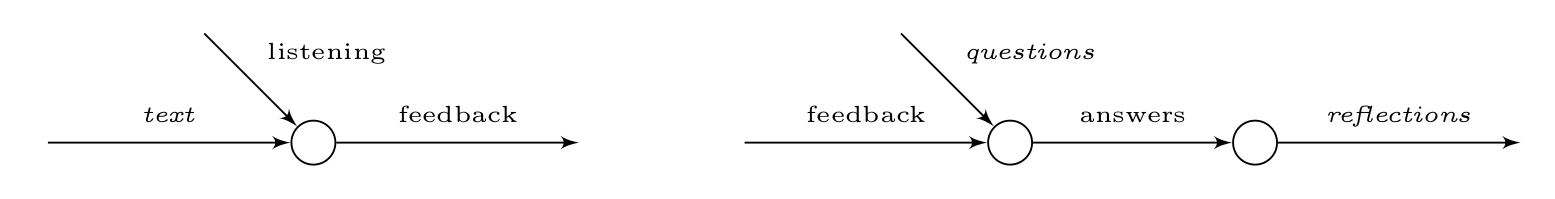
\includegraphics[width=.9\textwidth]{ww-serendipity-diagram}
%% \par}

Italicised elements (\emph{presentation}, \emph{questions}, and
\emph{reflections}) are the responsibilities of the presenting author,
and the upright elements (listening, feedback, and
answers) are the responsibilities of the attendant critics.
%
The system as a whole can be further decomposed into generative
components as follows:

\bigskip

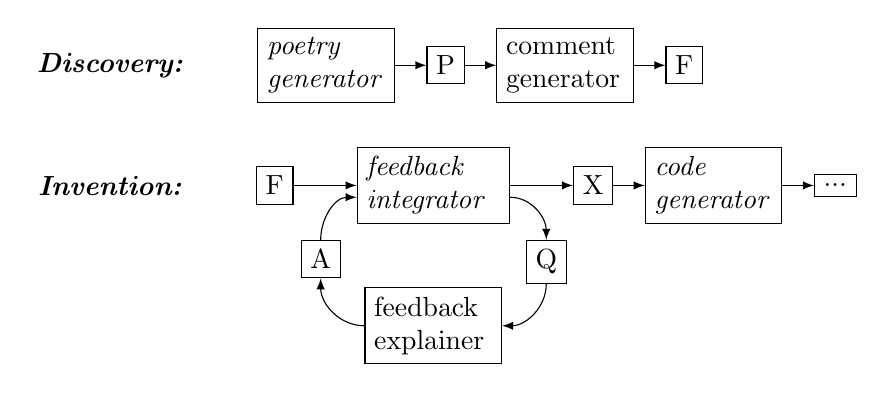
\begin{tikzpicture}[
single/.style={draw, anchor=text, rectangle},
]
\node (discovery) {\textbf{\emph{Discovery:}}};
% poet generates poem
\node[single, right=8mm of discovery.east,text width=1.5cm] (poet) {\emph{poetry generator}};
\node[single, right=4mm of poet.east] (poem) {P};
\draw [-latex] (poet.east) -- (poem.west);
% critic listens to poem and offers feedback
\node[single, right=4mm of poem.east,text width=1.5cm] (critic) {comment generator};
\draw [-latex] (poem.east) -- (critic.west);
\node[single, right=4mm of critic.east] (feedback) {F};
\draw [-latex] (critic.east) -- (feedback.west);

%%% Next phase
\node[below=1cm of discovery] (invention) {\textbf{\emph{Invention:}}};
% poet integrates feedback
\node[single, right=8mm of invention.east] (feedbackcont) {F};
\node[single, right=8mm of feedbackcont.east,text width=1.7cm] (integrator) {\emph{feedback integrator}};
\draw [-latex] (feedbackcont.east) -- (integrator.west);

\node[single, below=8mm of integrator.south,text width=1.5cm] (explainer) {feedback explainer};

\node[single, below right=2mm and 2mm of integrator] (question) {Q};
\node[single, below left=2mm and 2mm of integrator] (answer) {A};

\draw[-latex] ([yshift=-1.5mm]integrator.east) to [out=0,in=90] (question.north) ;
\draw[-latex] (question.south) to [out=270,in=0] (explainer.east) ;
\draw[-latex] (explainer.west) to [out=180,in=270] (answer.south) ;
\draw[-latex] (answer.north) to [out=90,in=180] ([yshift=-1.5mm]integrator.west) ;

\node[single, right=8mm of integrator.east] (problem) {X};

\draw [-latex] (integrator.east) -- (problem.west);

% poet reflects on feedback and updates codebase

\node[single, right=4mm of problem.east,text width=1.5cm] (pgrammer) {\emph{code}\\ \emph{generator}};

\draw [-latex] (problem.east) -- (pgrammer.west);

\node[single, right=4mm of pgrammer.east,text width=.3cm] (etc) {...};

\draw [-latex] (pgrammer.east) -- (etc.west);
\end{tikzpicture}


\bigskip

\noindent In our thought experiment, we focus on the case of hypothetical such discussions and exchange of views between computational poetry systems as our example of a situation where social circumstances could encourage serendipity. We note that similar
ideas would apply for prose and, with further adaptation, other arts.

\paragraph{Thought Experiment: Prepared mind.}
Participating systems need to be able to follow the protocol.  This
means that participating systems will need components like those
listed above. The {\tt listening} and {\tt questions} components of
the protocol correspond to $p$ and $p^{\prime}$ our model of
serendipity.  The corresponding ``comment generator'' and ``feedback
integrator'' modules in the architecture represent the primary points
of interface to the outside world.  In principle these modules need to
be prepared to deal (more or less thoughtfully) with \emph{any} text,
and in turn, with \emph{any} comment on that text.  Certain limits may
be agreed in advance; e.g.~as to genre or length in the case of texts,
and what constitutes an acceptable comment.  The ``feedback
explainer'' is closely connected with the ``comment generator'' and in
an implementation of this model they would presumably share a
codebase.  The loop for learning by asking questions as they arise is
reminiscent of the operating strategy of {\sf SHRDLU}
\cite{winograd1972understanding}.

\paragraph{Thought Experiment: Serendipity triggers.}

Although the poem is under the control of the initial generative
subsystem, it is \emph{not} under control of the listening subsystem.
The listening subsystem expects some poem, but it does not know what
poem to expect.  In this sense, the poem constitutes a serendipity
trigger $T$, not only for the listening subsystem, but for the
Workshop system as a whole.

To expand this point, note that there may be several listeners, each
sharing their own feedback and listening to the feedback presented by
others (which, again, is outside of their direct control).  This
creates further potential for serendipity, since each listener can
learn what others see in the poem.  More formally, in this case
$T^\star$ may seen as an evolving vector with shared state, but viewed
and handled from different perspectives.  With multiple agents
involved in the discussion, the ``comment generator'' module would
expand to contain its own feedback loops.

\paragraph{Thought Experiment: Bridge.}

Feedback on portions of the poem may lead the system to identify new
problems, indeed, new \emph{types} of problems that it hadn't
considered before.  The most immediately feasible case is one in which
the critic is a programmer who can directly program new concepts into
the computer \cite<cf.>{winograd1972understanding}.  However, it would
be hard to call that ``serendipity.''

We can also ask whether agents can build new concepts \emph{without}
outside intervention, starting with some basic concepts and abilities
related to poetry (e.g.~definitions of words, valence of sentiments,
metre, repetition, density, etc.) and code (e.g.~the data, functions,
and macros in which the poetic concepts and workshop protocols are
embodied).  Previous experiments with concept invention have been
fraught with questions about autonomy
\cite{ritchie1984case,lenat1984and}.  One cognitively inspired
hypothesis is that the formation of new concepts is closely related to
formation of sensory experiences \cite{milan2013kiki}.  If the
workshop participants have the capacity to identify the distinctive
features of a given poem, then training via a machine learning or
genetic algorithm approach could be used assemble a battery of
existing low-level tools that can approximate the effect.  Relatedly,
a compression process could seek to produce a given complex poetic
effect with a maximally-succinct algorithm.

The key point is that feedback on the poem -- simply describing what's
in the poem from several different points of view -- can be used to
define new problems for the system to solve.  This is not simply a
matter of decomposing the poem into pieces, but also of reconstructing
the way in which the pieces work together.  This is one of the
functions of the {\tt questions} step corresponding to $p^{\prime}$ in
our formalism: they offer the poet the opportunity to enquire about
how different pieces of feedback fit together, and learn more about
where they come from.  Although computers are currently nowhere close,
the reconstructive process may steadily approach the ideal case --
familiar to humans -- of relating to the sentiment expressed by the
poem as a whole \cite[p. 209]{bergson1983creative}.

%% Several of us are involved with a contemporary project
%% \cite{coinvent14} to develop a formal theory of concept invention,
%% focusing on \emph{concept blending}.  The additive or subtractive
%% blending of existing poetry profiles may be another way to create new
%% concepts.


%% should be possible Modifer Grammar
%% Counting Breathing Position Distribution Phonics Rhythm Repetition
%% Thematic Narrative Entropy

\paragraph{Thought Experiment: Result.} 

The final step is to take the problem or problems that were
identified, and write new code to solve them.  Several strategies for
generating a result $R$, in the form of new code, were described
above.  Now the system evaluates the new code to see whether it holds
promise.  In order to do this, it must have a way to carry out an
evaluation and judge whether $|R|>0$.  In the most straightforward
case, it would simply make changes to the draft poem that seem to
improve it in some way.  For example, the poet might remove or alter material that
elicited a negative response from a critic.  The system may proceed to
update its modules related to poetry generation.  Notably, it may also update its own
feedback modules, after reflecting on questions like: ``How might the
critic have detected that feature in my poem?''

We then develop several case studies (some historical and some imagined) showing
how serendipitous discovery+invention can work in a computational setting.
% 
\section{Discussion} \label{sec:discussion}

\subsection{Recommendations} \label{sec:recommendations}

In the diagrammatic formalism advanced in
\cite{colton-assessingprogress}, we spoke about progress with
\emph{systems} rather than with \emph{problems}.  It would be a useful
generalisation of the formalism -- and not just a simple relabelling
-- to tackle problems as well.
%
Figueiredo and Campos \cite{Figueiredo2001}, for example, describe
serendipitous ``moves'' from one problem to another.
%
However, progress with problems does not always mean transforming a
problem that cannot be solved into one that can.  Progress may also
apply to growth in the ability to posit problems.  As Deleuze writes:
``True freedom lies in the power to decide, to constitute problems
themselves'' \cite[p. 15]{deleuze1991bergsonism}.  Indeed, against any
education by means of ready-made problems, Dewey's perspective was
that
\begin{quote}
``\emph{the child's mind can be trained only in so far as the objects
    with which they are occupied arise out of their interests and
    their own problems.}''~\cite{dewey-by-mead}
\end{quote}

This was our emphasis in Section \ref{sec:unified-approach}:
developing new design patterns is closely connected with -- and in the
dynamical interpretation we prefer, effectively synonymous with --
positing new problems.  Although \cite{colton-assessingprogress}
presented a way to model creative progress at various levels of
granularity, it dealt primarily with \emph{solutions}; and although it
exhibited progress in a way that would be recognised by impartial
observers, the formalism did not focus on expositing the features that
would permit a system to actually \emph{make} creative progress.
Accordingly, we would recommend that in applying our earlier
formalism, system designers clearly record what problem a given system
solves, and the degree to which the computer was responsible for
coming up with this problem.

In \cite{stakeholder-groups-bookchapter}, we advanced a broader
programme for computational creativity, in which we argue in favour of
studying the \emph{perceptions} of creativity by various parties.  The
criteria developed in the current paper -- including the focus shift,
which we regard as fundamental -- can be used in the same way, as we
will describe below.

%% MC> Angelina is a able to read Twitter to find out what people think of
%% MC> people like Hamid Karzai, and then change the sorts of images that
%% MC> it finds as a result.  So you're going to see a happy picture of
%% MC> President Obama later next to a very angry picture of Hamid Karzai.
%% MC> While some of this might look creative and intelligent, a lot of it
%% MC> comes down to serendipity as well.  So the image you're about to see
%% MC> comes up for a Google search for terrorism that doesn't really have
%% MC> much relevance to the news article, and the sound that you're
%% MC> hearing now, the electronic drone, sounds like it's a good choice
%% MC> for a game that's about war and about feeling unsettling.  But in
%% MC> actuality I have no idea how Angelina came up with that choice.

Our proposed Writers Workshop is very different from the Turing-style
imitation game, but nevertheless may prove to be a useful aptitude
test for computer systems, and as a context in which computationally
creative programs may become aware of each other, and participate
actively in advancing the field of research.  We previously examined
perceptions of creativity in computational systems found among members
of the general public, Computational Creativity researchers, and
creative communities -- understood as human communities.  We should
now add a fourth important ``stakeholder'' group in computational
creativity research: computer systems themselves.

To make the point emphatically: the writers workshop proposed above is
very different from a traditional system ``Show and Tell'' presented
by system developers, for system developers.  Traditional academic
practices associated with presenting finished work, or even
work-in-progress, are not entirely suitable for the field of
computational creativity, where engagement between systems may exhibit
manifestly serendipitous results.  If the community does not implement
a suggestion like the one presented here, it will be missing out on a
key idea for enhancing computational creativity that has been
circulating since Turing suggested that computers should ``be able to
converse with each other to sharpen their wits''
\cite{turing-intelligent}.  Other fields, including computer Go
\cite{bouzy2001computer} and argumentation \cite{yuan2008towards} have
their own dedicated servers and protocols for exchange.  We should
move in that direction too.

There is ample room for unpredictability in such pursuits.  Creativity
may look very different to this fourth stakeholder group than it looks
to us.  In time to come, computer systems will increasingly take
leadership in matters of genre, interaction design, and their own
artistic and scientific training.  For now, our job is not at all to
get out of the way, like the parents of young adults, but rather to
participate in creating the ``play schools'' in which systems that are
quite frankly in early development can begin to socialise with each
other.
%
In \cite{stakeholder-groups-bookchapter}, we introduced nine
hypotheses related to the perception of creativity in computational
systems. 
The last of these hypotheses stated that:
\begin{quote}
``\emph{The perception of creativity in software which produces
  artefacts within a creative community will be increased if the
  software can exhibit subjective judgements about its own work and
  that of others, and defend those judgements in an accountable
  way.}''~\cite{stakeholder-groups-bookchapter}
\end{quote}
If the framework described in this paper is developed further, we may
be able to test this hypothesis in computer simulations.

Our proposed template for design patterns for participation in writers
workshops is different from, but complementary to Alexander's
framework.  Whereas Alexander focused on solutions to common
architectural problems (\emph{A place to wait}, etc.), our framework
is primarily designed to elicit and engage with new and unexpected
problems.  We presented four examples using the template, but our
intention is for the template to be used in a reflective mode by
systems to generate new patterns, in a manner appropriate to
second-order cybernetics.  Many practical issues remain to be settled
for a future computational enterprise that seeks to combine existing
design patterns and new stimuli in order to generate new, useful
design patterns.  One thing that becomes clear from this discussion is
that \emph{problem-setting} is a fundamental issue for the field of
computational creativity that will only be given due attention when
the research culture is ready to fully embrace serendipity.

\begin{quote}
``[S]\emph{ocial cybernetics must be a second-order cybernetics--a
    cybernetics of cybernetics--in order that the observer who enters
    the system shall be allowed to stipulate his own purpose: he is
    autonomous.}'' \cite[p. 286]{von2003essays}
\end{quote}

\subsection{Future Work} \label{sec:futurework}

From this, we extract recommendations for practitioners in computational creativity, and outline our own plan of work.
% \section{Conclusion} \label{sec:conclusion}

%
We began by surveying ``serendipity'', developing a broad historical
view, and describing several criteria for serendipity which we propose
to be computationally salient.  We reviewed related work; like
\citeA{andre2009discovery}, we propose a two-part definition of
serendipity: \emph{discovery} followed by \emph{invention}.
%
Adapting the ``Standardised Procedure for Evaluating Creative
Systems'' (SPECS) model from \citeA{jordanous:12}, we developed a set
of evaluation standards for serendipity.
%
We used this model to analyse prior examples of serendipity in the
context of evolutionary music improvisation and recommender systems,
and developed a thought experiment that seems able to support ``high
serendipity'' with a novel design for a computational poetry workshop.
%
We then reflected back over our definition, outlining a programme for
serendipitous computing in the pursuit of \emph{autonomy},
\emph{learning}, \emph{sociality}, and \emph{embedded evaluation}.  We
posit the following challenges, which connect with ongoing discussions
in the field:
%
\begin{itemize}
\item \emph{A primary challenge to the serendipitous operation of
  computers is developing computational agents that specify their own
  problems.}
\item \emph{A second challenge is for computational agents to learn
  more and more about the world we live in.}
\item \emph{A third challenge is for computational agents to interact
  in a recognisably social way with us and with each other, resulting
  in emergent effects.}
\item \emph{A fourth challenge is for computational agents to evaluate
  their own creative process and products.}
\end{itemize}
%
In the current work, we have limited ourselves to clarifying
conceptual issues surrounding our definition of serendipty, and
examining their design implications.
% 
We indicate several possible further directions for implementation
work in each of our case studies.  We have also drawn attention to
theoretical questions related to doing program design in an autonomous
programming context.  Our examples show that serendipity is not
foreign to computing practice.  There are further gains to be had for
research in computing by planning -- and programming -- for
serendipity.
%


\\[.5cm]
%
%% \keywords{serendipity,
%% design patterns,
%% intelligent machinery,
%% Writers Workshops}
\end{abstract}


\bigskip

\maketitle

% \linenumbers

\setcounter{footnote}{0}
%\tableofcontents
%\newpage
\section{Introduction}

Serendipity is centred on re-evaluation.  For example, a failed
attempt to develop an ultra-strong superglue resulted in a
re-stickable adhesive that no one was quite sure how to use.  After
considerable trial and error, this turned out to be just the right
ingredient for making the now ubiquitous Post-it\texttrademark\ notes.
%
% In this way, serendipity is related to deviations from expected or
% familiar patterns, and to new insight.
%
When we consider the practical uses for weak glue, the possibility
that a life-saving antibiotic might be found growing on contaminated
petri dishes, or the idea that burdock burrs could be anything but
annoying, we encounter radical changes in the evaluation of what's
interesting.  Importantly, serendipity is not the same as luck. 

The notion of serendipity is increasingly seen as relevant in the arts
\cite{mckay-serendipity}, in the tech industry \cite{rao2015breaking},
and elsewhere.  In the workplace, people have sought to encourage
serendipity with methods drawn from architecture, data science, and
cultural engineering
\cite{kakko2009homo,engineering-serendipity,who-moved-cube}.
Continued development of an interdisciplinary perspective on the
phenomenon of serendipity promises further illumination.  This paper
reassesses and updates an earlier discussion of serendipity in a
computational context.  \cite{pease2013discussion}.  Beginning with a
survey of historical definitions, perceptions, and examples of
serendipity in order to surface its several facets and features, we
then develop a process-based model of serendipity that can be applied
to system design and evaluation.

\citeA{van1994anatomy} -- echoing the
(negative) reflections on the potential
for a purely computational approach to mathematics from \citeA{poincare1910creation} -- claimed that:
\begin{quote}
``\emph{Like all intuitive operating, pure serendipity is not amenable
    to generation by a computer.  The very moment I can plan or
    programme `serendipity' it cannot be called serendipity
    anymore}.'' \cite[p.~646]{van1994anatomy}
\end{quote}
We believe that serendipity is not so mystical as such statements
might seem to imply.  In Section \ref{sec:discussion} we will show
that ``patterns of serendipity'' like those collected by van Andel can
be applied in the design of computational systems.  Purposive acts can
have unintended consequences \cite{merton1936unanticipated}.
Similarly, even if we cannot plan or program serendipity, we can
prepare for it.

If serendipity was ruled out as a matter of principle, computing would
be restricted to happy or unhappy \emph{unsurprises} -- preprogrammed,
preunderstood behaviour -- that would be interspersed periodically,
perhaps, with an \emph{unhappy} surprise.  (Perhaps this latter case
would ultimately reduce to ``programmer oversight''.)  Venkatesh Rao
\citeyearpar{rao2015breaking} uses the term \emph{zemblanity} -- after
William Boyd \citeyearpar{boyd2010armadillo}: ``zemblanity, the
opposite of serendipity, the faculty of making unhappy, unlucky and
expected discoveries by design'' -- to describe systems that are
doomed to produce only unhappy unsurprises.  According to Rao, this is
the implied fate of systems that are tied inextricably to a fixed
vision, from which any deviation constitutes a mistake.  This condition
stands at a sharp contrast with the ``second-order cybernetics''
introduced by \citeA{von2003cybernetics}, which envisions systems that
are able to specify their own purpose, and adapt it with respect to a
wider environment.  It also contrasts with Taleb's
\citeyearpar{taleb2012antifragile} notion of ``antifragility'' in
which disturbances within a certain range strengthen the system.
\citeA{minsky1967programming} argues that any sufficiently complex
computational system is bound to make decisions that its creators
could not foresee, and may not fully understand.  Demonstrably
gracefully behaviour in response to unexpected circumstances, and a
preference for ``happy'' as opposed to ``unhappy'' outcomes may be
prerequisites for the development of autonomous systems that are
worthy of our trust.  While not the same as ``Serendipity as a
Service'', such systems should at least be able to recognise
serendipity when it is happening.  Over time a system might also come
to recognise previous missed opportunities and false realisations --
what van Andel \citeyearpar[p.~639]{van1994anatomy} terms \emph{negative
  serendipity} -- and learn from them.

Less controversial than ``programmed serendipity'', but no less worthy
of study, is serendipity that arises in the course of user
interaction.  Indeed, it could be argued that everyday social media
already offers something approaching ``Serendipity as a Service''.
The user logs on hoping, but without any guarantee, that they will
find something interesting, charming, or entertaining, and potentially
relevant to whatever is going on in their life at the moment.
Of course, it should not be assumed that any system that can accommodate
user interaction can generate serendipity; take for example the use of
a calculator, where the potential for serendipity through user
interaction is minimal.  The frameworks introduced in this paper are
broad enough to be used in the design and evaluation of sociotechnical
systems, and we will touch on some examples, however we focus on
modelling serendipity in a computational context.

Section \ref{sec:literature-review} surveys the broad literature on
serendipity including the etymology of the term itself.  Section
\ref{sec:by-example} assembles a novel catalog of historical examples
of serendipity that we will use to scaffold our model.  In Section
\ref{sec:our-model} we present our own definition of serendipity,
which synthesises the understanding gained from these historical
examples, and prepares the way for evaluation of serendipity in
computational systems.  Section \ref{sec:computational-serendipity}
examines three such case studies.  Section \ref{sec:discussion}
examines prior applications of the concept of serendipity in
computing, and offers recommendations for researchers working in the
computational modelling of serendipity and related areas such as
computational creativity.  It also describes our own plans for future
work.  Section \ref{sec:conclusion} reviews the contributions of this
paper towards computational modelling and evaluation of serendipity.




\section{Literature review} \label{sec:literature-review}

\subsection{Etymology and selected definitions} \label{sec:overview-serendipity}  
The English term ``serendipity'' derives from the 1302 long poem \emph{Eight Paradises}, written in Persian by the Sufi poet Am\={\i}r Khusrow in Uttar Pradesh, India.  After translations into Italian, French, and finally English, its first chapter was known as ``The Three Princes of Serendip'', where ``Serendip'' ultimately corresponds to the Old Tamil-Malayalam word for Sri Lanka (%{\tam சேரன்தீவு},
\emph{Cerantivu}, island of the Ceran kings).
%
The term ``serendipity'' is first found in a 1757 letter by Horace Walpole to Horace Mann:
\begin{quote}
\emph{``This discovery is almost of that kind which I call serendipity, a very expressive
word} \ldots \emph{You will understand it better by the derivation than by the
definition. I once read a silly fairy tale, called The Three Princes of Serendip:
as their Highness travelled, they were always making discoveries, by accidents
\& sagacity, of things which they were not in quest of}[.]''~\cite[p. 633]{van1994anatomy}
\end{quote}
The same story formed part of the inspiration for Voltaire's \emph{Zadig}, and ``the method of Zadig'' was used as a term of art in 19th Century philosophy of science \cite{huxley1894science}.
Walpole's term ``serendipity'' was had been used in print only 135 times up until the 1958, according to the survey carried out by Robert Merton and Elinor Barber, collected in \emph{The Travels and Adventures of Serendipity} \citep{merton}.  Merton describes his own understanding of a generalised ``serendipity pattern'' and its constituent parts as follows:

\begin{quote}
``\emph{The serendipity pattern refers to the fairly common experience of observing an \emph{\textbf{unanticipated}}, \emph{\textbf{anomalous}} \emph{\textbf{and strategic}} datum which becomes the occasion for developing a new theory or for extending an existing theory.}''~\cite[p. 506]{merton1948bearing}~{[}emphasis in original{]}
    %% The datum [that exerts a pressure for initiating theory] is, first of all, unanticipated. A research directed toward the test of one hypothesis yields a fortuitous by-product, an unexpected observation which bears upon theories not in question when the research was begun.
    %% Secondly, the observation is anomalous, surprising, either because it seems inconsistent with prevailing theory or with other established facts. In either case, the seeming inconsistency provokes curiosity; it stimulates the investigator to "make sense of the datum," to fit it into a broader frame of knowledge....
    %% And thirdly, in noting that the unexpected fact must be "strategic," i. e., that it must permit of implications which bear upon generalized theory, we are, of course, referring rather to what the observer brings to the datum than to the datum itself. For it obviously requires a theoretically sensitized observer to detect the universal in the particular. 
\end{quote}

In 1986, Philippe Qu\'eau described serendipity as ``the art of
finding what we are not looking for by looking for what we are not
finding'' (\citeA{eloge-de-la-simulation}, as quoted in
\cite[p. 121]{Campos2002}).  Campbell
\citeyear{campbell2005serendipity} defines it as ``the rational
exploitation of chance observation, especially in the discovery of
something useful or beneficial.''  Pek van Andel
\citeyear[p. 631]{van1994anatomy} describes it simply as ``the art of
making an unsought finding.''


Roberts \citeyear[pp. 246--249]{roberts} records 30 entries for the term ``serendipity'' from English language dictionaries dating from 1909 to 1989.  
%
Classic definitions require the investigator not to be aware of the problem they serendipitously solve, but this criterion has largely dropped from dictionary definitions. Only 5 of Roberts' collected definitions explicitly say ``not sought for.''  Roberts characterises ``sought findings'' in which the discovery nevertheless follows from an accident as \emph{pseudoserendipity}, after \citeA{chumaceiro1995serendipity}.
%
While Walpole initially described serendipity as an event
(i.e., a kind of discovery), it has
since been reconceptualised as a psychological attribute, a matter of
sagacity on the part of the discoverer: a ``gift'' or ``faculty.''
Only one of Roberts collected definitions defined it solely as an event, while five define it as both
event and attribute.

Nevertheless, numerous historical examples exhibit features of
serendipity and develop on a social scale rather than an individual
scale.  For instance, between Spencer Silver's creation of high-tack,
low-adhesion glue in 1968, Arthur Fry's invention of a sticky bookmark in 1973,
and the eventual launch of the distinctive canary yellow re-stickable
notes in 1980, there were many opportunities for
Post-it\texttrademark\ Notes \emph{not} to have come to be
\cite{tce-postits}.  Merton and Barber argue that the
psychological perspective needs to be integrated with a
sociological perspective.
\begin{quote}
``\emph{For if chance favours prepared minds, it particularly favours
    those at work in microenvironments that make for unanticipated
    sociocognitive interactions between those prepared minds. These
    may be described as serendipitous sociocognitive
    microenvironments.}'' \cite[p. 259--260]{merton}
\end{quote}
Large-scale scientific and technical projects generally rely on the
convergence of interests of key actors and on other cultural factors.
For example, Umberto Eco describes the
historical role of serendipitous mistakes and falsehoods in the
production of knowledge \citeyear{eco2013serendipities}.

It is important to note that serendipity is usually discussed within
the context of \emph{discovery}, rather than \emph{creativity},
although in everyday parlance the latter two terms are closely related
\cite{jordanous12jims}.  In the definition of serendipity that we present in Section \ref{sec:our-model}, we make use
of Henri Bergson's distinction:
\begin{quote}
%% \emph{``La d\'ecouverte porte sur ce qui existe d\'ej\`a, actuellement
%%   ou virtuelle­ment ; elle \'etait donc s\^ure de venir t\^ot ou
%%   tard. L'invention donne l'\^etre \`a ce qui n'\'etait pas, elle
%%   aurait pu ne venir jamais.''}
``\emph{Discovery, or uncovering, has to do with what already exists,
    actually or virtually; it was therefore certain to happen sooner
    or later.  Invention gives being to what did not exist; it might
    never have happened.}''~\cite[p. 58]{bergson2010creative}
\end{quote}
As we have indicated, serendipity would seem to require features of
both discovery and invention: that is, the \emph{discovery} of
something unexpected in the world and the \emph{invention} of an
application for the same.  \citeA{mckay-serendipity} draws on the same
Bergsonian distinction to frame her argument about the role of
serendipity in artistic practice, where discovery and invention can be
seen as ongoing and diverse.  This underscores the relationship
between serendipity and creativity.

Following \citeA{austin2003chase}, \citeA{cropley2006praise} understands serendipity to
describe the case of a person who ``stumbles upon something novel and
effective when not looking for it.''  Nearby categories are
\emph{blind luck}, the \emph{luck of the diligent} (or
pseudoserendipity) and \emph{self-induced luck}; however, Cropley
questions ``whether it is a matter of luck at all'' because of the
work and knowledge involved in the process of assessment.
%
The perspective developed here sharpens these understandings in two ways:
firstly, we point out that work is involved in both phases of the process (even when chance plays a role), and secondly, following Bergson we defer true ``novelty'' to the invention phase.
%% In other words, serendipity involves creative making.  Furthermore, we
%% emphasise the importance of active, agential discernment over more
%% passive stumbling.

%% According to Arthur Cropley, creative thinking involves:
%% \begin{quote}
%% ``{[}N{]}\emph{ovelty generation followed by (or accompanied by) exploration of the novelty from the point of view of workability, acceptability, or similar criteria, in order to determine if it is effective.}'' \cite{cropley2006praise}
%% \end{quote}

We can point to process-level parallels between definitions of
serendipity like Merton's, quoted above, and previous definitions of
creativity.  Cs\'ikszentmih\'alyi's understanding of creativity within
a social context, for example:
\begin{quote}
``{[}C{]}\emph{reativity results from the interaction of a system
    composed of three elements: a culture that contains 
   \emph{\textbf{symbolic rules}}, a person who brings 
    \emph{\textbf{novelty}} into the symbolic domain, and a
    field of experts who recognize and 
    \emph{\textbf{validate}} the innovation.}''
  \cite[p.~6]{csikszentmihalyi1997flow}~{[}emphasis added{]}
\end{quote}
%% Although there are common features to existing definitions of
%% creativity, and again, much in common with serendipity,
%% there is also much disagreement and discussion -- for example,
%% about the relevance of the social context.

A often-cited five-stage model of creativity, based on
\emph{preparation}, \emph{incubation}, \emph{insight},
\emph{evaluation}, followed by \emph{elaboration}
\citeA[pp.~79--80, after \citeA{wallas1926art}]{csikszentmihalyi1997flow}
is particularly similar to the model of serendipity that we develop in
Section \ref{sec:our-model}.
%%
However, this is a parallel and not an equivalence.
We will adapt a general-purpose framework for evalutating creative
systems \cite{jordanous:12} to use in evaluating a system's potential
for serendipity.  These evaluations assume that several relatively
generic criteria may be measured.  The following section surveys those
criteria.
 
%\subsection{Serendipity by example} \label{sec:by-example}

We adapt the conceptual framework for describing serendipity proposed
by \citeA{pease2013discussion}.  This section will briefly introduce
the relevant concepts, and illustrate them by means of historical
examples of serendipity.

\subsubsection*{Key condition for serendipity.}

Serendipity relies on a reassessment or reevaluation -- a \emph{focus shift} in which something that was previously uninteresting, of neutral, or even negative value, becomes interesting.

\begin{itemize}
\item \textbf{Focus shift}: George de Mestral, an electrical engineer
  by training, and an experienced inventor, returned from a hunting
  trip in the Alps.  He removed several burdock burrs from his clothes
  and his dog's fur and became curious about how they worked. After
  examining them under a microscope, he realised the possibility of
  creating a new kind of fastener that worked in a similar fashion,
  laying the foundations for the hook-and-loop mechanism in Velcro\texttrademark.
% \cite[p. x]{roberts}
\end{itemize}

\subsubsection*{Components of serendipity.}

A focus shift is brought about by the meeting of a \emph{serendipity trigger} and a \emph{prepared mind}.  The next step involves building a \emph{bridge} to a valuable \emph{result}.

\begin{itemize}
\item \textbf{Prepared mind}: 
Fleming's ``prepared mind'' included his focus
on carrying out experiments to investigate influenza as well as his
previous experience that showed that foreign substances in petri dishes can kill
bacteria.  He was concerned above all with the question ``Is there a
substance which is harmful to harmful bacteria but harmless to human
tissue?''  \cite[p. 161]{roberts}.
\end{itemize}

\begin{itemize}
\item \textbf{Serendipity trigger}: The trigger does not directly
  cause the outcome, but rather, inspires a new insight.  It was long
  known by Quechua medics that cinchona bark stops shivering.  In
  particular, it worked well to stop shivering in malaria patients, as
  was observed when malarial Europeans first arrived in Peru.  The
  joint appearance of shivering Europeans and a South American remedy
  was the trigger.  That an extract from cinchona bark can cure and
  can even prevent malaria was learned subsequently.
\end{itemize}

\begin{itemize}
\item \textbf{Bridge}: The bridge often includes reasoning techniques,
  such as abductive inference (what might cause a clear patch in a
  petri dish?); analogical reasoning (de Mestral constructed a target
  domain from the source domain of burrs hooked onto fabric); and
  conceptual blending (Kekul\'e, discoverer of the benzene ring
  structure, blended his knowledge of molecule structure with his
  vision of a snake biting its tail).  The bridge may also rely on new
  social arrangements, such as the formation of cross-cultural
  research networks.
\end{itemize}

\begin{itemize}
\item \textbf{Result}: This may be a new product, artefact, process,
  hypothesis, a new use for a material substance, and so on.  The
  outcome may contribute evidence in support of a known hypothesis, or
  a solution to a known problem.  Alternatively, the result may itself
  {\em be} a new hypothesis or problem.  The result may be
  ``pseudoserendipitous'' in the sense that it was {\em sought}, while
  nevertheless arising from an unknown, unlikely, coincidental or
  unexpected source.  More classically, it is an \emph{unsought}
  finding, such as the discovery of the Rosetta stone.
\end{itemize}

\subsubsection*{Dimensions of serendipity.}

The four components described above have attributes that may be present to a greater or lesser degree.  These are: \emph{Chance} -- how likely was the trigger to appear?; \emph{Curiosity} -- how likely was this trigger to be identified as interesting?; \emph{Sagacity} -- how likely was it that the interesting trigger would be turned into a result?; -- and \emph{Value} (how valuable is the result that is ultimately produced?).

\begin{itemize}
\item \textbf{Chance}: Fleming \citeyear{fleming} noted: ``There are
  thousands of different moulds'' -- and ``that chance put the mould
  in the right spot at the right time was like winning the Irish
  sweep.''  It is important to notice that \emph{he} was in the right
  spot at the right time as well -- and that this was not a complete
  coincidence.  The chance events we're interested in always include
  at least one observer.
\end{itemize}

\begin{itemize}
\item \textbf{Curiosity}: Curiosity can dispose a creative person to
  begin or to continue a search into unfamiliar territory.  We use
  this word to describe both simple curiosity and related deeper
  drives.  Charles Goodyear \citeyear{goodyear1855gum} reflects on his
  own life experience as follows: ``[F]rom the time his attention was first given
  to the subject, a strong and abiding impression was made upon his
  mind, that an object so desirable and important, and so necessary to
  man's comfort, as the making of gum-elastic available to his use,
  was most certainly placed within his reach.  Having this
  presentiment, of which he could not divest himself, under the most
  trying adversity, he was stimulated with the hope of ultimately
  attaining this object.''
\end{itemize}

\begin{itemize}
\item \textbf{Sagacity}: This old-fashioned word is related to
  ``wisdom,'' ``insight,'' and especially to ``taste'' -- and
  describes the attributes, or skill, of the discoverer that
  contribute to forming the bridge between the trigger and the result.
  \citeA{merton1948bearing} writes: ``{[}M{]}en had for centuries
  noticed such `trivial' occurrences as slips of the tongue, slips of
  the pen, typographical errors, and lapses of memory, but it required
  the theoretic sensitivity of a Freud to see these as strategic data
  through which he could extend his theory of repression and
  symptomatic acts.''
\end{itemize}

%% Note that the chance ``discovery'' of, say, a \pounds 10 note may
%% be seen as happy by the person who finds it, whereas the loss of
%% the same note would generally be regarded as unhappy.

\begin{itemize}
\item \textbf{Value}: 
  Positive judgements of serendipity by a third party would be less
  likely in scenarios in which ``One man's loss is another man's
  gain'' than in scenarios where ``One man's trash is another man's
  treasure.''  One quite literal example is the Swiss
  company Freitag, started by design students who built a business
  around ``upcycling'' used truck tarpaulins into bags and backpacks.
  Thanks in part to clever marketing \cite[pp. 54--55,
    68--69,]{russo2010companies}, their product has sold well.
  Wherever possible, we prefer an independent judgement of value
  \cite{jordanous:12}.
\end{itemize}

\subsubsection*{Environmental factors.}

Finally, serendipity seems to be more likely for agents who experience and participate in a \emph{dynamic world}, who are active in \emph{multiple contexts}, occupied with \emph{multiple tasks}, and who avail themselves of \emph{multiple influences}.

\begin{itemize}
\item \textbf{Dynamic world}: Information about the world develops
  over time, and is not presented as a complete, consistent whole.  In
  particular, \emph{value} may come later.  Van Andel
  \citeyear[p. 643]{van1994anatomy} estimates that in twenty percent
  of innovations ``something was discovered before there was a demand
  for it.''  To illustrate the role of this factor, it may be most
  revealing to consider a counterexample, in a case where dynamics
  were not attended to carefully and the outcome suffered as a result.
  Cropley \citeyear{cropley2006praise} describes the pathologist Eugen
  Semmer's failure to recognise the importance of the role of
  \emph{penicillium notatum} in restoring two unwell horses to health:
  ``Semmer saw the horses' return to good health as a problem that
  made it impossible for him to investigate the cause of their death,
  and reported \ldots\ on how he had succeeded in eliminating the
  mould from his laboratory!''  This example shows that knowledge is
  not the only relevant condition for mental preparedness: the
  investigator also needs to have a suitable frame of mind, one that
  is ready to make a jump into the unknown as the world changes.  In a
  certain sense it is necessary to be able to ``overcome'' situated
  cognition, or at least be ready to revise the plan as the situation
  changes \cite{bereiter1997situated}.
\end{itemize}

\begin{itemize}
\item \textbf{Multiple contexts}: One of the dynamical aspects at play
  may be the discoverer going back and forth between different
  contexts with different stimuli.  3M employee Arthur Fry sang in a
  church choir and needed a good way to mark pages in his hymn book;
  he happened to have been attending seminars offered by his colleague
  Silver about restickable glue.
\end{itemize}

\begin{itemize}
\item \textbf{Multiple tasks}: Even within what would typically be
  seen as a single context, a discoverer may take on multiple tasks
  that segment the context into sub-contexts, or that cause the
  investigator to look in more than one direction.  The tasks may have
  an interesting \emph{overlap}, or they may point to a \emph{gap} in
  knowledge.  For example, Penzias and Wilson used a
  large antenna to detect radio waves that were relayed by bouncing
  off of satellites.  After they had removed interference effects due
  to radar, radio, and heat, they found residual ambient noise that
  couldn't be eliminated.
\end{itemize}

\begin{itemize}
\item \textbf{Multiple influences}: The bridge from trigger to
  result is often found by making use of a social network, thus, 
  Penzias and Wilson only understood the significance of their work
  after reading a preprint by Jim Peebles that hypothesised the
  possibility of measuring radiation released by the big bang.
\end{itemize}

\noindent We will show how the key condition, components,
dimensions and environmental factors of serendipity can be modelled
and assessed in computational systems in Sections \ref{sec:our-model}
and \ref{sec:computational-serendipity}.


\subsection{Serendipity by example: the condition, components, dimensions, and factors of serendiptious occurrences} \label{sec:by-example}

% This section introduces key concepts for understanding serendipitous occurrences, and illustrates them by means of historical examples.
%% We adapt the conceptual framework proposed by
%% \citeA{pease2013discussion}.

\subsubsection{Key condition for serendipity.}

Serendipity relies on a reassessment or reevaluation -- a \emph{focus shift} in which something that was previously uninteresting, of neutral, or even negative value, becomes interesting.

\begin{itemize}
\item \textbf{Focus shift}: George de Mestral, an electrical engineer
  by training, and an experienced inventor, returned from a hunting
  trip in the Alps.  He removed several burdock burrs from his clothes
  and his dog's fur and became curious about how they worked. After
  examining them under a microscope, he realised the possibility of
  creating a new kind of fastener that worked in a similar fashion,
  laying the foundations for the hook-and-loop mechanism in Velcro\texttrademark.
% \cite[p. x]{roberts}
\end{itemize}

\subsubsection{Components of serendipity.}

A focus shift is brought about by the meeting of a \emph{serendipity trigger} and a \emph{prepared mind}.  The next step involves building a \emph{bridge} to a valuable \emph{result}.

\begin{itemize}
\item \textbf{Prepared mind}: 
Alexander Fleming's ``prepared mind'' included his focus
on carrying out experiments to investigate influenza as well as his
previous experience that showed that foreign substances in petri dishes can kill
bacteria.  He was concerned above all with the question ``Is there a
substance which is harmful to harmful bacteria but harmless to human
tissue?''  \cite[p. 161]{roberts}.
\end{itemize}

\begin{itemize}
\item \textbf{Serendipity trigger}: The trigger does not directly
  cause the outcome, but rather, inspires a new insight.  It was long
  known by Quechua medics that cinchona bark stops shivering.  In
  particular, it worked well to stop shivering in malaria patients, as
  was observed when malarial Europeans first arrived in Peru.  The
  joint appearance of shivering Europeans and a South American remedy
  was the trigger.  That an extract from cinchona bark can cure and
  can even prevent malaria was learned subsequently.
\end{itemize}

\begin{itemize}
\item \textbf{Bridge}: The bridge often includes reasoning techniques,
  such as abductive inference (what might cause a clear patch in a
  petri dish?); analogical reasoning (de Mestral constructed a target
  domain from the source domain of burrs hooked onto fabric); and
  conceptual blending (Kekul\'e, discoverer of the benzene ring
  structure, blended his knowledge of molecule structure with his
  vision of a snake biting its tail).  The bridge may be
  non-conceptual, relying on new social arrangements, or physical
  prototypes.  It may have many steps, and, like the trigger, it may
  feature chance elements.  Several serendipitous episodes may be
  chained together in sequence, on the way to an unprecedented result.
  C\'edric Villani \citeyear[p.~16]{birth-of-a-theorem} describes a hallway
  conversation with his colleague \'Etienne Ghys, who said ``I didn't
  really want to say anything, C\'edric, but those figures there on
  the board -- I've seen them before.''
\end{itemize}

\begin{itemize}
\item \textbf{Result}: This is the new product, artefact, process,
  theory, use for a material substance, or other outcome.  The
  outcome may contribute evidence in support of a known hypothesis, or
  a solution to a known problem.  Alternatively, the result may itself
  {\em be} a new hypothesis or problem.  The result may be
  ``pseudoserendipitous'' in the sense that it was {\em sought}, while
  nevertheless arising from an unknown, unlikely, coincidental or
  unexpected source.  More classically, it is an \emph{unsought}
  finding, such as the discovery of the Rosetta stone.
\end{itemize}

\subsubsection{Dimensions of serendipity.}

The four components described above have attributes that may be present to a greater or lesser degree.  These are: \emph{Chance} -- how likely was the trigger to appear?; \emph{Curiosity} -- how likely was this trigger to be identified as interesting?; \emph{Sagacity} -- how likely was it that the interesting trigger would be turned into a result?; -- and \emph{Value} (how valuable is the result that is ultimately produced?).

\begin{itemize}
\item \textbf{Chance}: Fleming \citeyear{fleming} noted: ``There are
  thousands of different moulds'' -- and ``that chance put the mould
  in the right spot at the right time was like winning the Irish
  sweep.''  It is important to notice that \emph{he} was in the right
  spot at the right time as well -- and that this was not a complete
  coincidence.  The chance events we're interested in always include
  at least one observer.
\end{itemize}

\begin{itemize}
\item \textbf{Curiosity}: Curiosity can dispose a creative person to
  begin or to continue a search into unfamiliar territory.  We use
  this word to describe both simple curiosity and related deeper
  drives.  Charles Goodyear \citeyear{goodyear1855gum} reflects on his
  own life experience as follows: ``[F]rom the time his attention was first given
  to the subject, a strong and abiding impression was made upon his
  mind, that an object so desirable and important, and so necessary to
  man's comfort, as the making of gum-elastic available to his use,
  was most certainly placed within his reach.  Having this
  presentiment, of which he could not divest himself, under the most
  trying adversity, he was stimulated with the hope of ultimately
  attaining this object.''
\end{itemize}

\begin{itemize}
\item \textbf{Sagacity}: This old-fashioned word is related to
  ``wisdom,'' ``insight,'' and especially to ``taste'' -- and
  describes the attributes, or skill, of the discoverer that
  contribute to forming the bridge between the trigger and the result.
  \citeA{merton1948bearing} writes: ``{[}M{]}en had for centuries
  noticed such `trivial' occurrences as slips of the tongue, slips of
  the pen, typographical errors, and lapses of memory, but it required
  the theoretic sensitivity of a Freud to see these as strategic data
  through which he could extend his theory of repression and
  symptomatic acts.''
\end{itemize}

%% Note that the chance ``discovery'' of, say, a \pounds 10 note may
%% be seen as happy by the person who finds it, whereas the loss of
%% the same note would generally be regarded as unhappy.

\begin{itemize}
\item \textbf{Value}: Serendipity concerns happy surprises, but
  readings of a given situation as ``happy'' or ``surprising'' may be
  different for different parties.  A third party judgement of value
  can help to discriminate between mere luck and actual value
  creation.  Consider the difference between the two sayings ``One
  man's loss is another man's gain'' and ``One man's trash is another
  man's treasure.''  In the first case, it is unlikely that new value
  has been created, whereas the second case evokes a non-zero sum.
  A literal example of this second scenario is provided by the
  Swiss company Freitag, which was started by design students who
  built a business around ``upcycling'' used truck tarpaulins into
  bags and backpacks.  Thanks in part to clever marketing
  \cite[pp. 54--55, 68--69,]{russo2010companies}, their product is now
  a global brand.  Wherever possible, we prefer to make use of an
  independent judgement of value \cite{jordanous:12}.
\end{itemize}

\subsubsection{Environmental factors.}

Finally, serendipity seems to be more likely for agents who experience and participate in a \emph{dynamic world}, who are active in \emph{multiple contexts}, occupied with \emph{multiple tasks}, and who avail themselves of \emph{multiple influences}.

\begin{itemize}
\item \textbf{Dynamic world}: Information about the world develops
  over time, and is not presented as a complete, consistent whole.  In
  particular, \emph{value} may come later.  Van Andel
  \citeyear[p. 643]{van1994anatomy} estimates that in twenty percent
  of innovations ``something was discovered before there was a demand
  for it.''  To illustrate the role of this factor, it may be most
  revealing to consider a counterexample, in a case where dynamics
  were not attended to carefully and the outcome suffered as a result.
  Cropley \citeyear{cropley2006praise} describes the pathologist Eugen
  Semmer's failure to recognise the importance of the role of
  \emph{penicillium notatum} in restoring two unwell horses to health:
  ``Semmer saw the horses' return to good health as a problem that
  made it impossible for him to investigate the cause of their death,
  and reported \ldots\ on how he had succeeded in eliminating the
  mould from his laboratory!''  This example shows that knowledge is
  not the only relevant condition for mental preparedness: the
  investigator also needs to have a suitable frame of mind, one that
  is ready to make a jump into the unknown as the world changes.  In a
  certain sense it is necessary to be able to ``overcome'' situated
  cognition, or at least be ready to revise the approach as the
  situation changes \cite{bereiter1997situated}.
\end{itemize}

\begin{itemize}
\item \textbf{Multiple contexts}: One of the dynamical aspects at play
  may be the discoverer going back and forth between different
  contexts with different stimuli.  3M employee Arthur Fry sang in a
  church choir and needed a good way to mark pages in his hymn book;
  he happened to have been attending seminars offered by his colleague
  Silver about restickable glue.
\end{itemize}

\begin{itemize}
\item \textbf{Multiple tasks}: Even within what would typically be
  seen as a single context, a discoverer may take on multiple tasks
  that segment the context into sub-contexts, or that cause the
  investigator to look in more than one direction.  The tasks may have
  an interesting \emph{overlap}, or they may point to a \emph{gap} in
  knowledge.  For example, Penzias and Wilson used a
  large antenna to detect radio waves that were relayed by bouncing
  off of satellites.  After they had removed interference effects due
  to radar, radio, and heat, they found residual ambient noise that
  couldn't be eliminated.
\end{itemize}

\begin{itemize}
\item \textbf{Multiple influences}: The bridge from trigger to
  result is often found by making use of a social network, thus, 
  Penzias and Wilson only understood the significance of their work
  after reading a preprint by Jim Peebles that hypothesised the
  possibility of measuring radiation released by the big bang.
\end{itemize}

\noindent We will show how the key condition, components,
dimensions and environmental factors of serendipity can be modelled
and assessed in computational systems in Sections \ref{sec:our-model}
and \ref{sec:computational-serendipity}.

% \subsection{Related work} \label{sec:related}

An active research community investigating computational models of serendipity exists in the field of information retrieval, and specifically, in recommender systems \cite{Toms2000}. In this domain, \citeA{Herlocker2004} and \citeA{McNee2006} view serendipity as an important factor for user satisfaction, alongside accuracy and diversity.  Serendipity in recommendations is
understood to imply that the system suggests \emph{unexpected} items, which the user considers to be \emph{useful}, \emph{interesting}, \emph{attractive} or \emph{relevant}. 
% \cite{Herlocker2004} \cite{Lu2012},\cite{Ge2010}.  
Definitions differ as to the requirement of \emph{novelty}; \citeA{Adamopoulos2011}, for example, describe systems that suggest items that may already be known, but are still unexpected in the current context.  While standardised measures such as the $F_1$-score or the (R)MSE are used to determine the \emph{accuracy} of a recommendation (i.e.~whether the recommended item is very close to what the user is already known to prefer), there is no common agreement on a measure for serendipity yet, although there are several proposals \cite{Murakami2008, Adamopoulos2011, McCay-Peet2011,iaquinta2010can}.
In terms of our model, these systems focus mainly on producing a \emph{serendipity trigger} and predicting the potential for serendipitous \emph{discovery} on the side of the user.  Intelligent user modeling could bring other components of serendipity into play, as we will discuss in Section \ref{sec:computational-serendipity}.

Recent work has examined related topics of \emph{curiosity}
\cite{wu2013curiosity} and \emph{surprise} \cite{grace2014using} in
computing.  This latter work seeks to ``adopt methods from the field
of computational creativity [$\ldots$] to the generation of scientific
hypotheses.''  This is an example of an effort focused on
computational \emph{invention}.

Paul Andr{\'e} et al.~\citeyear{andre2009discovery} have examined
serendipity from a design perspective.  Like us, these authors
proposed a two-part model encompassing ``the chance encountering of
information, and the sagacity to derive insight from the encounter.''
According to Andr\'e et al., the first phase is the one that has most
frequently been automated -- but they suggest that computational
systems should be developed that support both aspects.  They
specifically suggest to focus on representational features:
\emph{domain expertise} and a \emph{common language model}.

These features seem to exemplify
aspects of the \emph{prepared mind}.  However, as we mentioned above,
the \emph{bridge} is a distinct process that mental preparation can
support, but that it does not necessarily fully determine.  For example, participants in
a poetry workshop may possess a very limited understanding of each
other's aims or of the work they are critiquing, and may as a
consequence talk past one another to a greater or lesser degree --
while nevertheless finding the overall process of participating in the
workshop illuminating and rewarding (often precisely because
such misunderstandings elucidate poor communication choices!).
Various social strategies, ranging from Writers Workshops to open
source software, pair programming, and design charettes
\cite[p. 11]{gabriel2002writer} have been developed to exploit similar
emergent effects and to develop \emph{new} shared language.  We have
recently investigated the feasibility of using
designs of this sort in multi-agent systems that learn by sharing and
discussing partial understandings \cite{corneli2015computational,corneli2015feedback}.

\citeA{robot-rendezvous} develop a discussion of serendipitous
rendezvous in a multi-agent system for a graph exploration problem, in
which ``[h]aving more data about their colleagues, better decisions
are made about the potential serendipity path.''  This has some
similarity to the discursive scenario described above, and shows that
\emph{asymmetric partial knowledge} can support serendipitious
findings.  These examples suggest that a distinction between emergent
knowledge of other actors and knowledge about an underlying domain may
be useful -- although the distinction may be less relevant if
the underlying domain itself has dynamic and emergent features.
\emph{Social coordination} among human users of information systems is
a current research topic. \citeA{rubin2010everyday} point out that
naive end users often \emph{talk about} serendiptious occurrences,
which presents another route for research and evaluation.

The {\sf SerenA} system developed by Deborah Maxwell et al.~\citeyear{maxwell2012designing} offers a case study of several of the points discussed above.
This system is designed to support serendipitous discovery for its (human) users
\cite{forth2013serena}.  The authors rely on a process-based model of
serendipity \cite{Makri2012,Makri2012a} that is derived from user
studies, including interviews with 28 researchers, looking for
instances of serendipity from both their personal and professional
lives.  This material was coded along three dimensions:
\emph{unexpectedness}, \emph{insightfulness}, and \emph{value}.  This
research aims to support the process of forming bridging connections
from an unexpected encounter to a previously unanticipated but valuable
outcome.  The theory focuses on the acts of \emph{reflection}
that foment both the creation of a bridge and estimates of the
potential value of the result.
%
While this description touches on all of the features of our model, {\sf
  SerenA} largely matches the description offered by Andr{\'e} et
al.~\citeyear{andre2009discovery} of discovery-focused systems, in which
the user experiences an ``aha'' moment and takes the
creative steps to realise the result.  {\sf SerenA}'s primary computational method is to
search outside of the normal search parameters in order to engineer
potentially serendipitous (or at least pseudo-serendipitous)
encounters.
%% Another
%% earlier related example of this sort of system is {\sf Max}, created
%% by Figueiredo and Campos \citeyear{Campos2002}.  The user emailed {\sf
%%   Max} with an existing list of interests and {\sf Max} would return a
%% web page that might also be of interest.  Other systems with similar
%% support for serendipitous discovery involve searching for analogies
%% \cite{Donoghue2002,Donoghue2012}) as well as content \cite{Iaquinta2008}.

In recent joint work \cite{colton-assessingprogress}, we presented a
diagrammatic formalism for evaluating progress in computational
creativity.  It is useful to ask what serendipity would add to this
formalism, and how the result compares with other attempts to
formalise serendipity, notably Figueiredo and Campos's
\citeyear{Figueiredo2001} `Serendipity Equations'.  
Figueiredo and Campos describe serendipitous ``moves'' from one
problem to another, which transform a problem that cannot be solved
into one that can.  In our diagrammatic formalism, we spoke about
progress with \emph{systems} rather than with \emph{problems}.  It
would be a useful generalisation of the formalism -- and not just a
simple relabelling -- for it to be able to tackle problems as well.
However, it is important to notice that progress with problems does not always mean transforming a
problem that cannot be solved into one that can.  Progress may also
apply to growth in the ability to \emph{posit} problems.  In keeping
track of progress, it would be useful for system designers to record
(or get their systems to record) what problem a given system solves,
and the degree to which the computer was responsible for coming up
with this problem.

As \citeA[p. 69]{pease2013discussion} remark, anomaly detection and
outlier analysis are part of the standard machine learning toolkit --
but recognising \emph{new} patterns and defining \emph{new} problems
is more ambitious.  Establishing complex analogies between evolving problems and
solutions is one of the key strategies used by teams of human designers
\cite{Analogical-problem-evolution-DCC}.  Kazjon Grace
\citeyear{kaz-thesis} presents a computational model of the creation
of new concepts and interpretations, but this work did include the
ability to create new higher order relationships necessary for complex
analogies.  New patterns and higher-order analogies were considered in
Hofstadter and Mitchell's {\sf Copycat} and the subsequent {\sf
  Metacat}, but these systems operated in a simple and fairly abstract
``microdomain''
\cite{hofstadter1994copycat,DBLP:journals/jetai/Marshall06}.  %% More
%% recent work in this tradition is surveyed in
%% \cite{eric-nichols-thesis}.

The relationship between serendipity and novel problems receives
considerable attention in the current work, since we want to
increasingly turn over responsibility for creating and maintaining a
prepared mind to the machine.



\section{A computational model of serendipity} \label{sec:our-model}

Figure \ref{fig:model} recapitulates the ideas from the previous
section, integrating them into a computationally meaningful model of
process.  The model is summarised in text form at the end of this
section, in our working definition of serendipity.

Figure \ref{fig:1a} is a heuristic map of the features of serendipity
introduced in Section \ref{sec:by-example}.
%
Dashed paths ending in `\ymark' show some of the things that can go
wrong.  A serendipity trigger might not arise, or might not attract
interest.  If interest is aroused, a path to a useful result may not
be sought, or may not be found.  If a result is
developed, it may turn out to be of little value.  Prior experience
with a related problem could be informative, but could also hamper
innovation.  Similarly, multiple tasks, influences, and
contexts can help to foster an inventive frame of mind, but they may
also be distractions.

Figure \ref{fig:1b} removes these unserendipitous paths to focus on
the key features of ``successful'' serendipity.
%
The \textbf{serendipity trigger} is denoted here by $T$.  
%
The \textbf{prepared mind} corresponds to those preparations, labeled
$p$ and $p^{\prime}$, that are relevant to the discovery and invention
phases, respectively.  These preparations may include training,
current attitude, access to relevant knowledge sources, and so on.
%
A \textbf{focus shift} takes place when the trigger is observed to be
interesting.  The now-interesting trigger is denoted $T^\star$, and is
common to both the discovery and the invention phases.
%
%
The \textbf{bridge} is comprised of the actions based on $p^{\prime}$
that are taken on $T^\star$ leading to the \textbf{result} $R$, which is ultimately given a positive evaluation.

\afterpage{\clearpage}
\begin{figure}[p]
\vspace{2mm}
\begin{minipage}[b]{\textwidth}
{\centering
\resizebox{1.02\textwidth}{!}{
\begin{tikzonimage}[width=.45\textwidth,angle=270]{figures/model-diagram/serendipity-attractor-bw}%[tsx/show help lines]
\node (dynamic)[rotate=90] at (-.02, .25) {\emph{dynamic world}};
\node (trigger) at (.05, .255) {\textbf{trigger}};
\node (chance) at (.045, .165) {chance};
\node (bridge) at (.46, .83) {\textbf{bridge}};
\node (result) at (.055, .665) {\textbf{result}};
\node (result)[text width=2cm,align=center] at (.7, .71) {\textbf{prepared mind}};
\node (focus) at (.95, .86) {{\bf \textsc{focus shift}}};
\node (curiosity)[rotate=35] at (.44,.58) {curiosity};
\node (sagacity)[rotate=-30] at (.72,.45) {sagacity};
\node (value) at (.04, .77) {value};
\node (influences)[text width=2cm,align=center,rotate=30] at (.99, .60) {{\small\baselineskip=2pt \emph{multiple influences}\par}};
\node (tasks)[text width=1.5cm,align=center,rotate=30] at (.85, .39) {{\small\baselineskip=2pt \emph{multiple tasks}\par}};
\node (contexts)[text width=1.5cm,align=center,rotate=30] at (.545, .47) {{\small\baselineskip=2pt \emph{multiple contexts}\par}};
\draw[-latex] (.05,.03) -- (.15,.03) node [midway, above] {\itshape{\scshape{discovery}}};
\draw[-latex] (.95,.03) -- (.85,.03) node [midway, above] {\itshape{\scshape{invention}}};
%% Adding an arrowhead
\draw[-{Latex[width=2mm]}] (-.001,.6265) -- (-.003,.6265);
% \node (begin1) at (-.02,.303) {\handmark};
\node (yes1) at (-.02,.6265) {\sunmark};
\node (no1) at (1.005, .165) {\ymark};
\node (no2) at (1.005, .3) {\ymark};
\node (no3) at (.63, .32) {\ymark};
\node (no4) at (0.003, .525) {\ymark};
\end{tikzonimage}

}


\par}
\vspace{-4mm}
\subcaption{A heuristic map, showing serendipitous and unserendipitous outcomes}\label{fig:1a}
\end{minipage}
\medskip

%%%%%%%%%%%%%%%%%%%%%%%%%%%%%%%%%%%%%%%%%%%%%%%%%%%%%%%%%%%%%%%%%%%%%%%%%%%%%%%%%%%%%%%%%%%%%%%%%%%%
\begin{minipage}[b]{\textwidth}
{\centering
\begingroup
\tikzset{
block/.style = {draw, fill=white, rectangle, minimum height=3em, minimum width=3em},
tmp/.style  = {coordinate}, 
sum/.style= {draw, fill=white, circle, node distance=1cm},
input/.style = {coordinate},
output/.style= {coordinate},
pinstyle/.style = {pin edge={to-,thin,black}}
}

\begin{tikzpicture}[auto, node distance=2cm,>=latex']
    \node [sum] (sum1) {};
    \node [input, name=pinput, above left=.7cm and .7cm of sum1] (pinput) {};
    \node [input, name=tinput, left of=sum1] (tinput) {};
    \node [input, name=minput, below left of=sum1] (minput) {};
    \node [input, name=minput, right of=sum1] (moutput) {};
    \draw [->] (pinput) -- node{$p$} (sum1);
    \draw [->] (tinput) -- node{\vphantom{{\tiny g}}$T$} (sum1);
    \draw [->] (sum1) -- node{\vphantom{{\tiny g}}$T^{\star}$}  (moutput);
\end{tikzpicture}
\hspace{1cm}
\begin{tikzpicture}[auto, node distance=2cm,>=latex']
    \node [sum] (sum1) {};
    \node [input, name=pinput, above left=.7cm and .7cm of sum1] (pinput) {};
    \node [input, name=tinput, left of=sum1] (tinput) {};
    \node [input, name=minput, below left of=sum1] (minput) {};
    \node [sum, right of=sum1] (sum2) {};
    \node [input, name=minput, right of=sum2] (moutput) {};
    \draw [->] (pinput) -- node{$p^{\prime}$} (sum1);
    \draw [->] (tinput) -- node{\vphantom{{\tiny g}}$T^{\star}$} (sum1);
    \draw [->] (sum1) -- node{\vphantom{{\tiny g}}$R$} (sum2);
    \draw [->] (sum2) -- node{$|R|>0$}  (moutput);
\end{tikzpicture}
\endgroup


%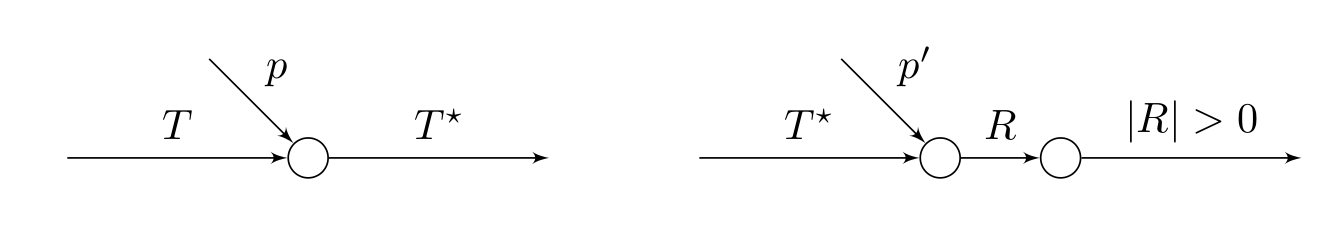
\includegraphics[width=.8\textwidth]{schematic}
\par}
\subcaption{A simplified process schematic, showing the key features of the model}\label{fig:1b}
\end{minipage}
\medskip

%%%%%%%%%%%%%%%%%%%%%%%%%%%%%%%%%%%%%%%%%%%%%%%%%%%%%%%%%%%%%%%%%%%%%%%%%%%%%%%%%%%%%%%%%%%%%%%%%%%%
\begin{minipage}[b]{\textwidth}
{\centering
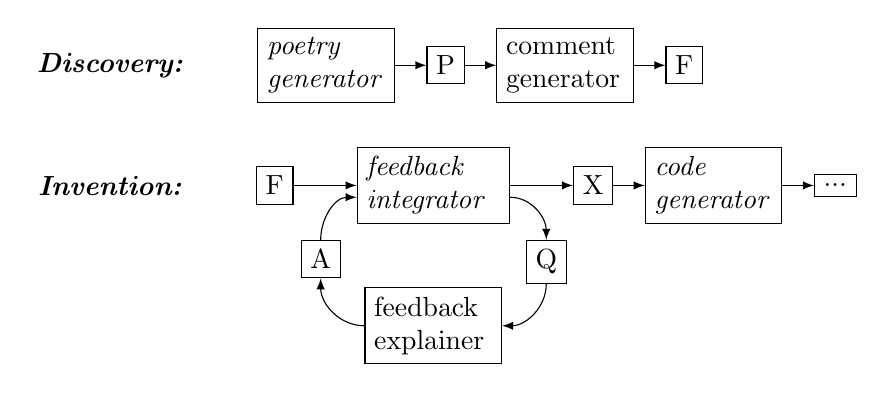
\begin{tikzpicture}[
single/.style={draw, anchor=text, rectangle},
]
\node (discovery) {\textbf{\emph{Discovery:}}};
% poet generates poem
\node[single, right=8mm of discovery.east,text width=1.5cm] (poet) {\emph{poetry generator}};
\node[single, right=4mm of poet.east] (poem) {P};
\draw [-latex] (poet.east) -- (poem.west);
% critic listens to poem and offers feedback
\node[single, right=4mm of poem.east,text width=1.5cm] (critic) {comment generator};
\draw [-latex] (poem.east) -- (critic.west);
\node[single, right=4mm of critic.east] (feedback) {F};
\draw [-latex] (critic.east) -- (feedback.west);

%%% Next phase
\node[below=1cm of discovery] (invention) {\textbf{\emph{Invention:}}};
% poet integrates feedback
\node[single, right=8mm of invention.east] (feedbackcont) {F};
\node[single, right=8mm of feedbackcont.east,text width=1.7cm] (integrator) {\emph{feedback integrator}};
\draw [-latex] (feedbackcont.east) -- (integrator.west);

\node[single, below=8mm of integrator.south,text width=1.5cm] (explainer) {feedback explainer};

\node[single, below right=2mm and 2mm of integrator] (question) {Q};
\node[single, below left=2mm and 2mm of integrator] (answer) {A};

\draw[-latex] ([yshift=-1.5mm]integrator.east) to [out=0,in=90] (question.north) ;
\draw[-latex] (question.south) to [out=270,in=0] (explainer.east) ;
\draw[-latex] (explainer.west) to [out=180,in=270] (answer.south) ;
\draw[-latex] (answer.north) to [out=90,in=180] ([yshift=-1.5mm]integrator.west) ;

\node[single, right=8mm of integrator.east] (problem) {X};

\draw [-latex] (integrator.east) -- (problem.west);

% poet reflects on feedback and updates codebase

\node[single, right=4mm of problem.east,text width=1.5cm] (pgrammer) {\emph{code}\\ \emph{generator}};

\draw [-latex] (problem.east) -- (pgrammer.west);

\node[single, right=4mm of pgrammer.east,text width=.3cm] (etc) {...};

\draw [-latex] (pgrammer.east) -- (etc.west);
\end{tikzpicture}

%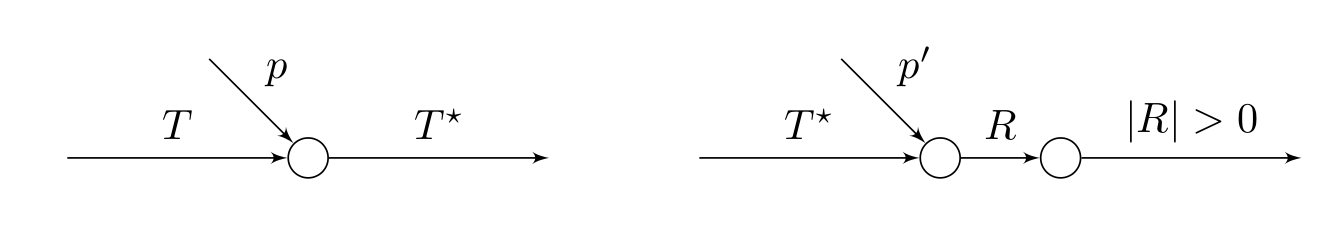
\includegraphics[width=.8\textwidth]{schematic}

\par}
\smallskip

\subcaption{A boxes-and-arrows diagram, showing one possible implementation architecture}\label{fig:1c}
\end{minipage}
\bigskip

\caption{Three representations of the elements of serendipity}\label{fig:model}
\end{figure}

Figure \ref{fig:1c} expands this schematic into a sketch of the
components of one possible idealised implementation of a serendipitous
system.  An existing \emph{generative process} is assumed.  This may
be based on observations of the outside world, or it may be a purely
computational process.  In any case, its products are passed on to the
next stage.  After running this data through a feedback loop, certain
aspects of the data are singled out, and marked up as
``interesting.''  Note that this designation need not arise all at
once: rather, it the outcome of a \emph{reflective process}.  In the
implementation envisioned here, this process makes use of two primary
functions: $p_1$, which notices particular aspects of the data, and $p_2$, which
offers reflections about those aspects.  Together, these functions build up a
``feedback object,'' $T^{\star}$, which consists of the original data
and further metadata.  This is passed on to an \emph{experimental
  process}, which has the task of verifying that the data
is indeed interesting, and determining what it may be useful for.
This is again an iterative process, relying on functions $p^{\prime}_1$ and $p^{\prime}_2$, which
build a contextual understanding of the trigger by devising experiments and
assessing their results.  Once implications or applications have been found, a result is
generated, which is passed to a final \emph{evaluation process}, and,
from there, to applications.

The ellipses at the end of the workflow in Figure \ref{fig:1c} are
intended to suggest that applications are open-ended; however, an
important class of applications will result in changes to one or more
of the system's modules, for example by expanding the knowledge base
that they have available.  Note that earlier components of the workflow
cannot, in general, anticipate what the subsequent phases will produce
or achieve.  If the system's next steps could be anticipated, we would
not say that the behaviour was serendipitous.  In other words,
serendipity does not adhere to one specific part of the system, but to
its operations as a whole.  Although Figures  \ref{fig:1b} and  \ref{fig:1c}
treat the case of successful serendipity, as indicated in Figure
 \ref{fig:1a}, each step is fallible, as is the system as a whole.
Thus, for example, a trigger that has been initially tagged as interesting may prove to be fruitless.
Similarly a system that implements all of the steps in Figure \ref{fig:1c}, but that never
achieves results of value does not have potential for serendipity.
However, a system only produces results of high value would also be
suspect, since it would indicate a tight coupling between trigger
and outcome.  Fallibility is a ``meta-criterion'' that transcends the criteria from Section \ref{sec:by-example}.
Summarising, we propose the following:

\begin{mdframed}
\begin{ndef}
\emph{(1) Within a system with a prepared mind, a previously uninteresting trigger arises due to circumstances that the system does not control and cannot predict, and is classified as interesting by the system; and,}
\emph{(2) The system uses the trigger and prior preparation, together with relevant computational processing, networking, and experimental techniques, to obtain a novel result that is evaluated favourably by the system or by external sources.}
\end{ndef}
\end{mdframed}



\subsection{Using SPECS to evaluate computational serendipity}\label{specs-overview}

In this section, we use the elements of the conceptual framework
described in Section \ref{sec:by-example} help to flesh out this
definition, to develop quite detailed evaluation criteria.
We adapt the \emph{Standardised Procedure for Evaluating Creative Systems} (SPECS),
a high-level, customisable evaluation strategy that was devised to judge the creativity
of computational systems \cite{jordanous:12}.  

In the three step SPECS process, the evaluator defines the concepts
and behaviours that signal creativity, converts this definition into
clear standards, and then applies them to evaluate the target systems.
%
We follow a slightly modified version of Jordanous's earlier evaluation
guidelines, in that rather than attempt a definition and evaluation of
{\em creativity}, we follow the three steps for \emph{serendipity}.

%\vspace{-.3cm}
\subsubsection*{Step 1: Identify a definition of serendipity that your system should satisfy to be considered serendipitous.}
%~\\
%\vspace{-.1cm}

\noindent We adopt the definition of serendipity from Section
\ref{sec:our-model}.

%\vspace{-.3cm}
\subsubsection*{Step 2: Using Step 1, clearly state what standards you use to evaluate the serendipity of your system.}
%~\\
%\vspace{-.1cm}

\noindent With our definition and other features of the model in mind, we propose the following standards for evaluating serendipity in computational systems. These criteria allow the evaluator to assess the degree of seredipity that is present in a given system's operation.

%% Serendipity relies on a reassessment or reevaluation -- a \emph{focus shift} in which something that was previously uninteresting, of neutral, or even negative value, becomes interesting.

\begin{description}[itemsep=16pt]
\item[{(\textbf{A - Definitional characteristics})}] {The system can
  be said to have a {\textbf{prepared mind}}, consisting of previous
  experiences, background knowledge, a store of unsolved problems,
  skills, expectations, readiness to learn, and (optionally) a current
  focus or goal.  It then processes a {\textbf{trigger}} that is at
  least partially the result of factors outside of its control,
  including randomness or unexpected events.  It classifies this
  trigger as interesting, constituting a {\textbf{focus shift}}.  The
  system then uses reasoning techniques and/or social or otherwise
  externally enacted alternatives to create a {\textbf{bridge}} from
  the trigger to a result.  The {\textbf{result}} is evaluated as
  useful, by the system and/or by an external source.}  The evaluator
  should specify all of these aspects relative to the system under
  consideration at a sufficient degree of precision to show their
  processual interconnection.
%%%%%%%%%%%%%%%%%%%%%%%%%%%%%%%%%%%%%%%%%%%%%%%%%%%%%%%%%%%%%%%%%%%%%
\item[{(\textbf{B - Dimensions})}] {Serendipity, and its various
  dimensions, can be present to a greater or lesser degree.  If the
  criteria above have been met, we consider the system (and
  optionally, generate ratings as estimated probabilities) along
  several dimensions:
%
{($\mathbf{a}$: \textbf{chance})} how likely was this trigger to appear to
  the system?
%
{($\mathbf{b}$: \textbf{curiosity})} On a population basis, comparing
similar circumstances, how likely was the trigger to be identified as
interesting?
%
{($\mathbf{c}$: \textbf{sagacity})} On a population basis, comparing
similar circumstances, how likely was it that the trigger would be
turned into a result?
%
Finally, we ask, again, comparing similar results where possible:
{($\mathbf{d}$: \textbf{value})} How valuable is the result that
is ultimately produced?}
%
%Then combining $\mathbf{a}\times\mathbf{b}\times\mathbf{c}$ gives a
 % likelihood score: 
{Low but nonzero likelihood $\mathbf{a}\times\mathbf{b}\times\mathbf{c}$ 
 and high value $\mathbf{d}$ are the criteria we use to say that the event was ``highly serendipitous.''}
%%%%%%%%%%%%%%%%%%%%%%%%%%%%%%%%%%%%%%%%%%%%%%%%%%%%%%%%%%%%%%%%%%%%%
\item[{(\textbf{C - Factors})}] {Finally, if the criteria from Part A
  are met, and if the event is deemed sufficiently serendipitous to
  warrant further investigation according to the criteria in Part B,
  then in order to deepen our qualitative understanding of the
  serendipitous behaviour, we ask: To what extent does the system
  exist in a {\textbf{dynamic world}}, spanning {\textbf{multiple
      contexts}}, featuring {\textbf{multiple tasks}}, and
  incorporating {\textbf{multiple influences}}?}
\end{description}

%\vspace{-.3cm}
\subsubsection*{Step 3: Test your serendipitous system against the standards stated in Step 2 and report the results.}
%~\\
%\vspace{-.1cm}

\noindent In Section \ref{sec:computational-serendipity}, we will pilot our framework by examining the degree of serendipity of existing and hypothetical computational systems. 

\subsection{Heuristics}\label{specs-heuristics}

How can we we estimate the chance of the trigger appearing, if every
trigger is unique?  Consider de Mestral's encounter with burrs.
The chance of encountering burrs while out walking is high: many
people have had that experience.  The unique features of de Mestral's
experience are that he had the curiosity to investigate the burrs
under a microscope, and the sagacity (and tenacity) to turn what he
discovered into a successful product.  The details of the particular
burrs that were encountered are essentially irrelevant.  This shows that it is not essential for all factors contributing to the likelihood score to be ``low'' in order for a given process of discovery and invention to be deemed serendipitous. In the general case, we are not interested in the chance of encountering a particular object or set of data.  Rather, we are interested the chance of encountering some trigger that could precipitate an interested response.  The trigger itself may be a complex object or event that takes place over a period of time; in other words, it may be a pattern, rather than a fact.  Noticing patterns is a key aspect of sagacity, as well.

Although it is in no way required by the SPECS methodology outlined
above, many systems (including all of the examples below) have an
iterative aspect.  This means that a result may serve as a trigger for
further discovery.  In such a case, further
indeterminacy may need to be introduced to the system, lest the results be
convergent, and therefor, infallible.  In applying the critera to
such systems, we consider long-term behaviour.



\section{Serendipity in computational systems} \label{sec:computational-serendipity}

The 13 facets of serendipity from Section \ref{sec:literature-review} specify the
conditions and preconditions that are conducive to serendipitous
discovery.  Section \ref{sec:our-model} distilled these elements into a computational model,
culminating in a method for evaluating computational serendipity in Section \ref{specs-overview}.
%
Along with clear criteria, it is important to clearly delineate the
scope of the system being evaluated, and the position of the evaluator
(recalling that ``embedded evaluation'' is a requisite part of a
serendipitous system).
For example, a standard spell-checking program might suggest a substitution that the user
deems especially fortuitous; and we might agree that serendipity has
occurred, but we would not locate the potential for serendipity in
the spell-checker itself, but rather to the ``cyborg'' system
comprised of the user plus the machine and its software.

\citeA{pease2013discussion} used an earlier variant the SPECS criteria
to analyse three examples of potentially serendipitous behaviour:
dynamic investigation problems, model generation, and poetry
flowcharts.  Using our updated criteria, we discuss two new examples
below, and revisit poetry flowcharts in our third example, reporting
on recent work.  As Campbell \citeyear{campbell2005serendipity}
writes, ``serendipity presupposes a smart mind,'' and these examples
suggest potential directions for further work in computational
intelligence.


%% If the system learns an $N$th fact or
%% If applied to a system which could be described as minimally
%% serendipitous at best, and perhaps not at all serendipitous, does our
%% model identify the lack or presence of serendipity?  
%% %% As example, a spellchecker
%% %% program identifies spelling errors in text input and optionally can
%% %% correct spelling automatically. The only situation we can conceive of
%% %% where serendipity could possibly occur is tenuous; perhaps a suggested
%% %% correction may be incorrect, but may lead the user to interpret the
%% %% correction in an unexpected way. In all other aspects that we have
%% %% considered, spellchecker software would be a decidedly unlikely
%% %% candidate for harbouring serendipitous opportunities.  
%% Traditional spellchecker programs could be said to have a
%% \textbf{prepared mind}, in that they are constructed with internal
%% dictionaries with which to check spelling and ways of deciding what a
%% misspelled word might be.  Given our above discussion of how the
%% system might be serendipitous, the \textbf{serendipity trigger} could
%% be seen as the user misspelling a word and the system suggesting
%% alternative possibilities that the user had not previously conceived.
%% However, the \textbf{bridge} from trigger to serendipitous result (if
%% any) would have been built by the user, not by the system.  With
%% adaptive context-aware text completion tools, we can imagine a
%% ``Cyrano de Bergero'' effect in which the machine finds a
%% serendipitous bridge and offers the \textbf{result} to the user.
%% However, the current generation of text completion tools are known
%% more for infelicities than for exceptional wit.

\subsection{Case Study: Evolutionary music improvisation} \label{sec:evomusic}

\citeA{jordanous10} reported a computational jazz improvisation system
(later given the name {\sf GAmprovising} \cite{jordanous:12}) that
uses genetic algorithms.  Reevaluating {\sf GAmprovising} can shed
light on the degree to which evolutionary computing can encourage
computational serendipity.

{\sf GAmprovising} uses genetic algorithms to evolve a population of \emph{Improvisors}. Each Improvisor is able to randomly generate music based on various parameters such as the range of notes to be used, preferred notes, rhythmic implications around note lengths and other musical parameters, see \cite{jordanous10}. These parameters are what define the Improvisor at any point in the system's evolution.  After a cycle of evolution, each Improvisor is evaluated using a fitness function based on Ritchie's \citeyear{ritchie07} formal criteria for creativity.  This model relies on user-supplied ratings of the novelty and appropriateness of the music produced by the Improvisor to calculate 18 metrics that collectively indicate how creative the system is.  The fittest Improvisors are used to seed a new generation of Improvisors, through crossover and mutation operations.

The {\sf GAmprovising} system can be said to have a \textbf{prepared mind} through its background knowledge of what musical concepts to embed in the Improvisors and the evolutionary abilities to evolve Improvisors. A potential \textbf{serendipity trigger} comes from the combination of previous mutation and crossover operations with current user input.  To be clear, in the current version of the system it is a human evaluator who is largely responsible for the system's \textbf{focus shift}, since the user tells the system which improvisations are most valuable.   \citeA{jordanous10}
notes that this ``introduces a fitness bottleneck.''  In future versions of the system, autonomous evaluation could potentially take over for the human evaluator.  Once the interesting samples have been collected (from whatever source), a \textbf{bridge} is then built to new results through the creation of new Improvisors.  The \textbf{results} are the various musical improvisations produced by the fittest Improvisors (as well as, perhaps, the parameters that have been considered fittest).

%% The likelihood of serendipitous evolution is greatly enhanced by the
%% use of random mutation and crossover operations within the genetic
%% algorithm, which increase the diversity of the search space covered by
%% the system during evolution.  
The probability of encountering any particular pair of Improvisor and
user evaluation is vanishingly low, given the massive dimensions of
this search space.  However, there will always be a highest-scoring
Improviser, whose parameters will be used to seed the next round.  Do
we estimate the \textbf{chance} of the trigger appearing according to
its uniqueness, or according to the system's attentive observation of
all triggers that cross its path?  Consider de Mestral's encounter
with burrs: the chance of encountering burrs while out walking was
high, and the details of the particular burrs that were encountered
effectively irrelevant.  The situation here is similar: despite their
uniqueness, the trigger appearing is ``high.''  The evolution of
Improvisors captures a sense of \textbf{curiosity} about how to
satisfy the musical tastes of a particular human user who identifies
certain Improvisors as interesting.  The \textbf{sagacity} of the
system corresponds to its methods for enhancing the likelihood that
the user will appreciate a given Improvisor's music (or similar music)
over time.  With little basis for comparison, we can only say that
these two dimensions are ``typical.''  The aim of the system is to
maximise the \textbf{value} of the generated results by employing a
fitness function, and indeed, the system:
\begin{quote}
``{[}W{]}\emph{as able to produce jazz
improvisations which slowly evolved from what was essentially random
noise, to become more pleasing and sound more like jazz to the human
evaluator's ears}'' \cite{jordanous10}.
\end{quote}
The very reliability of the
system ultimately bears against its overall serendipity.  Following
Step 2, Part B of the SPECS procedure, we find a likelihood measure of
$\mathit{high}\times\mathit{moderate}\times\mathit{moderate}$, with
outcomes of moderate value, so that the system as a whole is ``not
very serendipitous.''  Evaluating individual threads (as members
of a larger population) would yield varied results, which
emphasises the importance of system scoping, mentioned above.
However, it would be inaccurate to simply say that successful threads are serendipitous and unsuccessful threads are unserendipitous,  since that ignores contributing dimensions apart from value.  At the moment, individual threads are effectively equivalent regarding chance,
curiosity, and sagacity; a thread-by-thread analysis should be deferred until there would be more to say.

This is related to other changes that would improve the global serendipity score, as the following qualitative factor analysis indicates.
%
The {\sf GAmprovising} system does operate in \textbf{dynamic world},
assuming that the user's tastes may change.  A more elaborate version
of the system that could cater to multiple users is not yet
implemented, but would be occupied with a considerably more complex
problem, spanning and integrating \textbf{multiple contexts}.  The
system clearly engages with \textbf{multiple tasks}, but these are
largely separate, for instance, one global fitness function is used,
rather than evolving a local fitness function for each user along with
their ratings.  \textbf{Multiple influences} are present but currently
only at compile time, in the design of the fitness function, and the
selection of musical parameters that can later be set.  Greater
dynamism in future versions of the system would be likely to increase
its potential for serendipity.

\subsection{Case Study: Next-generation recommender systems} \label{sec:nextgenrec}
% Stress distinction between serendipity on the system- vs. serendipity on the user's side.
As discussed in Section \ref{sec:related}, recommender systems are one
of the primary contexts in computing where serendipity is currently discussed.  Serendipity, for current recommender systems, means suggesting items to a user that will be likely to introduce new ideas that are unexpected, but close to what the user is already interested in.  As we noted, these systems mostly focus on supporting \emph{discovery} for the user -- but some architectures also seem to take account of \emph{invention} of new methods for making recommendations, e.g.~using Bayesian methods, as surveyed in \citeNP{shengbo-guo-thesis}.  In light of our working definition of serendipity, we need to distinguish serendipity on the user side from serendipity in the system itself.

Current recommendation techniques focused on serendipity associate less popular items with high unexpectedness \cite{Herlocker2004,Lu2012}, and use clustering to discover latent structures in the search space, e.g., partitioning users into clusters of common interests, or clustering users and domain objects \cite{Kamahara2005,Onuma2009,Zhang2011}.  But even in the Bayesian case, the system has limited autonomy.  A case for giving more autonomy to recommender systems can be made, especially in complex and rapidly evolving domains where hand-tuning is cost-intensive or infeasible.

With this challenge in mind, we ask how serendipity could be achieved on the system side. In terms of our model, current systems have at least the makings of a \textbf{prepared mind}, comprising both a user- and a domain model, both of which can be updated dynamically.  User behaviour (e.g.~following certain recommendations) or changes to the domain (e.g.~adding a new product) may serve as a potential \textbf{trigger} that could ultimately cause the system to discover a new way to make recommendations in the future.  
In the current generation of systems that seek to induce serendipity for the user, the system provides a trigger for the user's focus shift by presenting recommendations that are neither too close, nor too far away from what user already knows; it is the other way around here. Note, however, that it is unexpected behaviour in aggregate, rather than a one-off event, that is likely to provide grounds for a \textbf{focus shift}.   
A \textbf{bridge} to a new kind of recommendation could be created by looking at exceptional patterns as they appear over time.  For instance, new elements may have been introduced into the domain that do not cluster well, or a user may suddenly indicate a strong preference towards an item that does not fit their preference history.  Clusters may appear in the user model that do not have obvious connections between them.  A new recommendation strategy that addresses the organisation's goals would be a serendipitous \textbf{result}.

The system has only imperfect knowledge of user preferences and
interests.  At least relative to current recommender systems, the
\textbf{chance} of noticing some particular pattern in user behaviour
seems quite low.  The urge to make recommendations specifically for
the purposes of finding out more about users could be described as
\textbf{curiosity}.  Such recommendations may work to the detriment of
other metrics over the short term.  In principle, the system's
curiosity could be set as a parameter, depending on how much coherence
is permitted to suffer for the sake of gaining new knowledge.
Measures of \textbf{sagacity} would relate to the system's ability to
develop useful experiments and draw sensible inferences from user
behaviour.  For example, the system would have to select the best time
to initiate an A/B test.  A significant amount programming would have
to be invested in order to make this sort of judgement call
autonomously, so such systems are understandably rare.  The
\textbf{value} of recommendation strategies can be measured in terms
of traditional business metrics or other organisational objectives.
In this case, we compute a likelihood measure of
$\mathit{low}\times\mathit{variable}\times\mathit{low}$, with outcomes
of potentially high value, so that such a system is ``potentially
highly serendipitous.''

Recommender systems have to cope with a \textbf{dynamic world} of changing user preferences and a changing collection of items to recommend.  A dynamic environment which exhibits some degree of regularity represents a precondition for useful A/B testing.  The system's \textbf{multiple contexts} include the user model, the domain model, as well as an evolving model of its own organisation.  A system matching the description here would have \textbf{multiple tasks}: making useful recommendations, generating new experiments to learn about users, and improving its models.  In order to make effective decisions, a system would have to avail itself of \textbf{multiple influences} related to experimental design, psychology, and domain understanding.  Pathways for user contributions that go beyond answers to the question ``Was this recommendation helpful?'' could be one way make the relevant expertise available.

\subsection{Case Study: Automated flowchart assembly} \label{sec:flowchartassembly}

Here we consider the design of a contemporary experiment with the
{\sf FloWr} flowcharting framework \cite{colton-flowcharting}.  {\sf FloWr} is a
tool for creating and runnable flowcharts, built of small
modules called ProcessNodes.  For day-to-day user, {\sf FloWr} functions as a visual programming environment.  However, it can also be invoked programmatically, on the Java Virtual Machine, or with any language
using a new web API.  The goals of {\sf FloWr} are both to be a user
friendly tool for co-creativity, and to be an autonomous
\emph{Flowchart Writer}.  Our experiment targets the latter scenario,
assembling available ProcessNodes into flowcharts automatically.  This can be viewed as a simple example of automated programming.

In the backend, {\sf FloWr}'s flowcharts are stored as scripts.  These
detail the names of the involved nodes together with their (input)
parameters and (output) variable settings.  Connections between nodes
are established when one node's input parameter references the output
variable of another node.
%
Inputs and outputs have constraints.  For instance, the {\tt
  WordSenseCategoriser} node has a {\tt stringsToCategorise}
parameter, which needs to be seeded with an ArrayList of strings.  The node produces useful output only when these strings can be parsed as as a space-separated list of words.  Similarly, the node's {\tt requiredSense} parameter needs to be seeded with a string that represents one of the 57 British National Corpus Part of Speech tags.  Given constraints of this nature, the first challenge in automated flowchart assembly is to match inputs to outputs correctly, and to make sure that all required inputs are satisfied.

In our current experiment, the system's potential \textbf{triggers}
result from random, but constrained, trial and error with flowchart assembly.  Some valid
combinations of nodes will produce results, and some will not.  Due to
the dynamically changing environment (e.g., updates to data sources
like Twitter) some flowcharts that did not produce results earlier may
unexpectedly begin to produce results.
%
The system's \textbf{prepared mind} lies in a distributed knowledge
base provided by ProcessNodes, showing the constraints on their inputs
and outputs; and in the global history of successful and unsuccessful combinations.
%
The system will not try combinations that it knows cannot produce
results, but it will try novel combinations and may retry earlier
flowchart specimens that have the chance to become viable.  Turning a
collection of nodes for which no known working combination existed
into a working flowchart is an occasion for a \textbf{focus shift}:
what made this particular combination work?  Is there a pattern that
could be exploited in the future?  It may be that no
broader pattern can be found, other than the fact that the combination works.
%
Successful combinations and any further inferences are stored, and
referred to in future runs.  The \textbf{bridge} to any new
results is accordingly found by informed trial and error, building
on previous outcomes.
%
In these early experiments, the basic \textbf{result} the system is
aiming to achieve is simply to generate a new combination of nodes that can fit together and that generate non-empty output.  Subsequent versions of the system may have more detailed evaluation functions, setting a higher bar.  For example, a future version of the system could be tuned to search for flowcharts that generate poetry \cite{corneli2015computational}.

The \textbf{chance} of finding a novel successful flowchart in any given sample of nodes is fairly low.  Compared to
humans users of {\sf FloWr}, the search process is exceptionally \textbf{curious}, since tries many combinations programmatically.  However, remembering viable combinations and avoiding combinations that are known not to work offer only a modest degree of \textbf{sagacity}.  At the moment,
the system's criterion for attributing \textbf{value} is simply that
the combination of nodes generates non-empty output; an
third-party is not likely to judge these combinations as
useful.  The associated likelihood score is
$\mathit{low}\times\mathit{low}\times\mathit{high}$, which
is relatively favourable.  However, until there is a
more discriminating way to judge value, the attribution of serendipity to any particular run may be premature.  One route
would be to attribute value to explanatory heuristics, rather
than generated texts; this would require increased sagacity on
the part of the system as well.

The \textbf{dynamic world} the system operates in is dynamic in two
ways: first, in the straightforward sense that some of the input
sources, like Twitter, are changing; and also in the sense that the
system's knowledge of successful and unsuccessful node combinations
changes over time.  The current version of the system does not seem to
deal with \textbf{multiple contexts}; even though we have broken the
experiment into separate sub-populations to constrain the search,
these do not interact.  However, in a future version of the system,
interaction between different heuristically-driven search processes
would be possible, and could produce more unexpected results.  Along
these lines, as more goals are added, the system could more readily be
seen to have \textbf{multiple tasks}.  For instance, one search
process could look for narrative outlines to structure a poem with,
and another process could look for lines or stanzas to fill out that
outline.  As for \textbf{multiple influences}, the population of
ProcessNodes will constrain (and, as more nodes are added, extend) the
possible strategies for assembling flowcharts.

\afterpage{\clearpage}
\begin{table}[p]
{\centering \renewcommand{\arraystretch}{1.5}
\scriptsize
\begin{tabular}{p{1.5in}@{\hspace{.1in}}p{1.5in}@{\hspace{.1in}}p{1.5in}}
\multicolumn{1}{c}{\textbf{{\footnotesize Evolutionary music}}} & \multicolumn{1}{c}{\textbf{{\footnotesize Next-gen.~recommenders\hspace{.4cm}}}} & \multicolumn{1}{c}{\textbf{{\footnotesize Flowchart assembly}}} \\[.05in]
\multicolumn{3}{l}{\em {\textbf{Condition}}} \\
\cline{1-3}
\multicolumn{3}{l}{\em Focus shift} \\[-.1cm]
Driven by (currently, human) evaluation of samples
& Unexpected behaviour in the aggregate
& Find a pattern to explain a successful combination of nodes\\
\cline{1-3}
~\\[-.1cm]
\multicolumn{3}{l}{\em {\textbf{Components}}} \\
\cline{1-3}
\multicolumn{3}{l}{\em Trigger} \\[-.1cm]
% \textbf{Trigger}
Previous evolutionary steps, in combination with user input
& Input from user behaviour
& Trial and error in combinatorial search \\
% \cline{1-3}
\multicolumn{3}{l}{\em Prepared mind} \\[-.1cm]
% \textbf{Prepared mind}
Musical knowledge, evolution mechanisms
& Through user/domain model
& Constraints on node inputs and outputs; history of successes and failures\\
% \cline{1-3}
%\textbf{Bridge}
\multicolumn{3}{l}{\em Bridge} \\[-.1cm]
Newly-evolved Improvisors
& Elements identified outside clusters
& Try novel combinations \\
% \cline{1-3}
%\textbf{Result}
\multicolumn{3}{l}{\em Result} \\[-.1cm]
Music generated by the fittest Improvisors
& Dependent on organisation goals
& Non-empty or more highly qualified output \\ \cline{1-3}
~\\[-.1cm]
%%%%%%%%%%%%%%%%%%%%%%%%%%%%%%%%%%%%%%%%%%%%%%%%%%%%%%%%%%%%%%%%%%%%%%%%%%%%%%%%%%%%%%%%%%%%%%%%%%%%
\multicolumn{3}{l}{\em \textbf{Dimensions}}  \\
\cline{1-3}
%\textbf{Chance}
\multicolumn{3}{l}{\em Chance} \\[-.1cm]
Looking for rare gems in a huge search space
& Imperfect knowledge of user preferences and behaviour
& Changing state of the outside world; random selection of nodes to try \\
% \cline{1-3}
%\textbf{Curiosity}
\multicolumn{3}{l}{\em Curiosity} \\[-.1cm]
Aiming to have a particular user take note of an Improvisor
& Making unusual recommendations
& Search for novel combinations \\
% \cline{1-3}
%\textbf{Sagacity}
\multicolumn{3}{l}{\em Sagacity} \\[-.1cm]
Enhance user appreciation of Improvisor over time,
using a fitness function
& Update recommendation model after user behaviour 
& Don't try things known not to work; consider variations on successful patterns \\
% \cline{1-3}
%\textbf{Value} &
\multicolumn{3}{l}{\em Value} \\[-.1cm]
Via fitness function (as a proxy measure of creativity)
& Per business metrics/objectives
& Currently ``non-empty results''; more interesting evaluation functions possible \\
\cline{1-3}
%%%%%%%%%%%%%%%%%%%%%%%%%%%%%%%%%%%%%%%%%%%%%%%%%%%%%%%%%%%%%%%%%%%%%%%%%%%%%%%%%%%%%%%%%%%%%%%%%%%%
~\\[-.1cm]
\multicolumn{3}{l}{\em \textbf{Factors}} \\
\cline{1-3}
%\textbf{Dynamic world}
\multicolumn{3}{l}{\em Dynamic world} \\[-.1cm]
Changes in the user tastes
& As precondition for testing system's influences on user behaviour
& Changing data sources and growing domain knowledge \\
%\cline{1-3}
%\textbf{Multiple contexts}
\multicolumn{3}{l}{\em Multiple contexts} \\[-.1cm]
Multiple users' opinions would change what the system is curious about and require greater sagacity
& User model, domain model, model of its own behaviour
& Interaction between different heuristic search processes would increase unexpectedness \\
% \cline{1-3}
%\textbf{Multiple tasks}
\multicolumn{3}{l}{\em Multiple tasks} \\[-.1cm]
Evolve Improvisors, generate music, collect user input, carry out fitness calculations
& Make recommendations, learn from users, update models
& Generate new heuristics and new domain artefacts \\
% \cline{1-3}
%\textbf{Multiple influences}
\multicolumn{3}{l}{\em Multiple influences} \\[-.1cm]
Through programming of fitness function and musical parameter combinations
& Experimental design, psychology, domain understanding
& Learning to combine new kinds of ProcessNodes\\
\cline{1-3}
\end{tabular}
\par}
\normalsize
\bigskip

\caption{Summary: applying our computational serendipity model to three case studies\label{caseStudies}}
\end{table}

\subsection{Summary}

Table \ref{caseStudies} summarises how the condition, components,
dimensions and factors in our model of serendipity appear in an
evolutionary music system, in hypothetical ``next-generation''
recommender systems, and in our current work on a flowchart-assembly
system.  Each of the case studies shows clear potential for
serendipity.  There are also clear ways in which the measure of
serendipity could be enhanced.

\begin{enumerate}
\item A future version of the evolutionary music system would be more
  convincingly sagacious if it could evaluate works without user
  intervention.  It might also be able to tailor its fitness function
  to the individual user.  More broadly, interaction between the
  system's tasks and more dynamism in its influences would help
  differentiate individual threads or system runs, and some elements
  of this population might be more serendipitous than others.

\item The next-generation recommender systems we've envisioned need to
  be able to make inferences from aggregate user behaviour.  This
  points to long-term considerations that go beyond the unique
  serendipitous event.  How ``curious'' should these systems be?  One
  obvious criterion is that short-term value should be allowed to
  suffer as long as expected value is still higher.  The symmetry
  between serendipity on the user side, and serendipity on the system
  side might be exploited.  Current systems seek to induce serendipity
  by making use of implicit connections between clusters, resulting in
  an update to the user's conception of the item space.  As in the
  example of {\sf SerenA} discussed in Section \ref{sec:related}, in
  current systems the user shares a significant part of the workload
  when forming the bridge, even when triggered by the system.  Users
  might be given the explicit task of triggering serendipity on the
  system-side, as well.

\item The flowchart assembly process would need more stringent, and
  more meaningful, criteria for value before third-party observers
  would be likely to attribute serendipity to the system.  In addition
  to raising challenges for autonomous evaluation (as in the
  evolutionary music system case), this requirement would impose more
  sophisticated constaints on processing in earlier steps, which would
  require the system to be more sagacious.
\end{enumerate}


\section{Discussion and Related Work} \label{sec:discussion}

In Section \ref{sec:computational-serendipity}, we applied our model
to evaluate the serendipity of an evolutionary music improvisation
system, a system for automatically assembling flowcharts, and
a hypothetical class of next-generation recommender systems.

The model has helped to highlight directions for development that
would increase a system's potential for serendipity, either
incrementally or more transformatively.  Our model outlines a path
towards the development of systems that can observe events that would
otherwise not be observed, take an interest in them, and transform the
observations into artefacts with lasting value.

%% In this section, we will show how the model allows for more precise
%% thinking than other existing work touching on this area.  We then
%% discuss implications from our findings for future research.

%\subsection{Challenges for future research} \label{sec:recommendations}

Viewing the concepts in Section \ref{sec:by-example} through the
practice scenarios we have discussed, we can describe the following
challenges for research in computational serendipity.

\begin{itemize}
\item \textbf{Autonomy}: Our case studies in Section \ref{sec:priorart} highlight the potential value of increased autonomy on the system side.
%% The thought experiment in Section
%% \ref{sec:ww} develops a design illustrating the relationship between
%% creativity at the level of artefacts (e.g.~new poems) and
%% creativity at the level of \emph{problem specification} (learning
%% new poetic concepts).
The search for connections that make raw data into ``strategic data''
is an appropriate theme for research in computational intelligence and
machine learning to grapple with.  In the standard cybernetic model,
we control computers, and we also control the computer's operating
context.  There is little room for serendipity if there is nothing
outside of our direct control.  In contrast with the mainstream model,
von Foerster \citeyear[p. 286]{von2003cybernetics} advocated a
\emph{second-order cybernetics} in which ``the observer who enters the
system shall be allowed to stipulate his own purpose.''  \emph{A
  primary challenge to the serendipitous operation of computers is
  developing computational agents that specify their own problems.}
\end{itemize}

\begin{itemize}
\item \textbf{Learning}: The Writers Workshop described in Section
  \ref{sec:ww} is one possible design for a system
  that can \emph{learn from experience}.  The Workshop model
  ``personifies'' the wider world in the form of one or several
  critics.  It is also possible for a lone creative agent to
  take its own critical approach in relationship to the world at
  large, using an experimental approach to generate feedback, and then
  looking for models to fit this feedback.   We are led to consider 
  computational agents that operate in our world rather
  than a circumscribed microdomain, and that are curious about this
  world.  \emph{A second challenge is for computational agents to
    learn more and more about the world we live in.}
\end{itemize}

\begin{itemize}
\item \textbf{Sociality}: We may be aided in our pursuit of the
  ``smart mind'' required for serendipity by recalling Turing's
  proposal that computers should ``be able to converse with each other
  to sharpen their wits'' \cite{turing-intelligent}.  Other fields,
  including computer Chess, Go, and argumentation have achieved this,
  and to good effect.  Turing recognised that computers would have to
  be coached in the direction of social learning, but that once they
  attain that standard they will learn much more quickly.  Deleuze
  \citeyear[p. 26]{deleuze1994difference} wrote: ``We learn nothing
  from those who say: `Do as I do'. Our only teachers are those who
  tell us to `do with me'[.]''  \emph{A third challenge is for
    computational agents to interact in a recognisably social way with
    us and with each other, resulting in emergent effects.}
\end{itemize}

\begin{itemize}
\item \textbf{Embedded evaluation}:
  \citeA{stakeholder-groups-bookchapter} outlined a general programme
  for computational creativity, and examined perceptions of creativity
  in computational systems found among members of the general public,
  Computational Creativity researchers, and existing creative
  communities.  We should now add a fourth important ``stakeholder''
  group in computational creativity research: computer systems
  themselves.  Creativity may look very different to this fourth
  stakeholder group than it looks to us.  It is our responsibility as
  system designers to teach our systems how to make
  evaluations in way that is both reasonable and ethical.  This is
  exemplified by the preference for a ``non-zero sum'' criterion for
  value suggested in our discussion of the dimensions of serendipity
  in Section \ref{sec:by-example}.  \emph{A fourth challenge is for
    computational agents to evaluate their own creative process and
    products.}
\end{itemize}


%% A survey of word occurrences from a recent special issue of
%% \emph{Cognitive Computation} on ``Computational Creativity, Intelligence and Autonomy'' \cite{bishop-erden-special-issue} shows that related themes are broadly
%% active in the research community.  Here
%% \emph{italics} indicates that the word stem accounted for 0.1\% of the
%% article or more; added \textbf{\emph{bold}} indicates that it
%% accounted for 1\% or more.\footnote{Articles were converted to text
%%   via {\tt pdftotext -layout}, individual counts found via {\tt tr
%%     \textquotesingle~\textquotesingle~\textquotesingle\textbackslash
%%     n\textquotesingle~< file.txt | grep -c "stem*"}, and total word counts
%%   via {\tt wc -w}.  The corresponding counts for the \emph{current}
%%   paper are 12, \emph{25}, \emph{16}, \emph{44} and 12.7K.}

%% \medskip

%% {\centering \setlength{\tabcolsep}{3pt} \footnotesize
\begin{tabular}{ccccccccccccccc}
paper \#
&1
&2
&3
&4
&5
&6
&7
&8
&9
&10
&11
&12
&13
&14
\\
\cline{2-15}
"autonom.*"
&0
&\textbf{\emph{32}}
&\emph{12}
&\emph{41}
&0
&1
&\emph{31}
&2
&1
&\emph{92}
&11
&2
&5
&\textbf{\emph{22}}
\\
"learn.*"
&6
&2
&2
&\emph{14}
&\emph{9}
&\textbf{\emph{118}}
&\emph{14}
&\emph{18}
&\emph{44}
&\emph{12}
&11
&\emph{42}
&\emph{44}
&2
\\
"social.*"
&0
&0
&\emph{23}
&\emph{25}
&0
&1
&2
&\emph{10}
&\emph{19}
&\emph{19}
&8
&\emph{21}
&13
&2
\\
"evaluat.*"
&0
&1
&\emph{11}
&\emph{20}
&0
&1
&3
&6
&4
&9
&8
&2
&\textbf{\emph{304}}
&0
\\
\cline{2-15}
total(K)
& 8.3  % &8337 (/ 6 8337.0)
& 2.2  % &2221 (/ 32 2221.0)  0.0135074290859973
& 7.5  % &7507  (/ 12 7507.0) 0.0015985080591447982 (/ 23 7507.0) 0.0026641800985746636 (/ 11 7507.0)0.001465299054216065
& 7.4  % &7453 (/ 41 7453.0) 0.004964443848114853 (/ 14 7453.0) 0.0009392191064001073 (/ 16 7453.0) 0.002146786528914531 (/ 19 7453.0) 0.0025493090030860054
& 8.6  % &8675 (/ 9 8675.0)
& 5.8  % & 5816 (/ 89 5816.0) 0.015302613480055021
&10.3 % &10341 (/ 30 10341.0) 0.002901073397156948
& 9.6  % &9632  (/ 18 9632.0) 0.0018687707641196014  (/ 10 9632.0)0.0010382059800664453
&10.8 % &10851 (/ 36 10851.0) 0.0033176665745092617
&11.6 % &11693 (/ 92 11693.0)0.007867955186863935 (/ 12 11693.0)
&14.4 % &14407 (/ 11 14407.0) 0.0007635177344346498
&10.8 % &10840 (/ 31 10840.0) 0.0028597785977859777
&25.3 % &25326 (/ 13  25326.0)  (/ 44  25326.0) 0.0008291873963515755 (/ 304 25326.0) 0.011174287293690278
& 1.6  % &1673 (/ 21 1673.0) 0.012552301255230125
\\
\end{tabular}
}


%% \bigskip

%% Paper 4, Rob Saunders's \citeyear{saunders2012towards} ``Towards
%% Autonomous Creative Systems: A Computational Approach'' was the only
%% contributed paper to emphasise all four of our themes according to the
%% metric above.  Saunders asks: ``What would it mean to produce an
%% autonomous creative system? How might we approach this task? And, how
%% would we know if we had succeeded?''  He argues for an approach ``that
%% models personal motivations, social interactions and the evolution of
%% domains.''  Paper 10, d'Inverno and Luck's \citeyear{d2012creativity}
%% ``Creativity Through Autonomy and Interaction'', also contains a
%% theoretical engagement with these themes, and presents a formalism for
%% multi-agent systems that could usefully be adapted to model
%% serendipitous encounters.  Both papers are particularly concerned with
%% \emph{motivation}, a topic that relates to both the prepared mind and
%% the theme of embedded evaluation.

%% We believe that our clarifications to the multifaceted concept of
%% serendipity will help encourage future computer-aided (and
%% computer-driven) investigations of the above themes and their
%% interrelationships.  Our extension of SPECS to cover serendipity will
%% be useful for evaluating progress.  We discuss some of our related
%% research plans below.

%\subsection{Future Work} \label{sec:futurework} \label{sec:hatching}

In looking for ways to manage and encourage serendipity, we are drawn
to the approach taken by the \emph{design pattern} community
\cite{alexander1999origins}.
%% The essential features of this approach
%% are described below, but we point out straight away that we propose to
%% use design patterns in rather nonstandard fashion.  These adaptations
%% to the typical design pattern methodology are proposed to parallel the
%% four themes outlined above.
%% \begin{itemize}
%% \item[(1)] We want to encode our design patterns directly in runnable
%%   programs, not just give them to programmers as heuristic guidance.
%% \item[(2)] We want the (automated) programmer to generate new design
%%   patterns, not just apply or adapt old ones.
%% \item[(3)] We want our design patterns themselves, working in
%%   combination, to contribute to the discovery of new emergent problems
%%   and patterns, not just capture the solutions to existing known
%%   problems.
%% \item[(4)] We want our design patterns to play an overt role in the
%%   dynamical systems they describe.
%% \end{itemize}
%%
\citeA{meszaros1998pattern} describe the typical scenario for authors of design
patterns: ``You are an experienced practitioner in your
field. You have noticed that you keep using a certain solution to a
commonly occurring problem. You would like to share your experience
with others.''  There are many ways to describe a solution.
Meszaros and Doble remark, ``What sets patterns apart is their
ability to explain the rationale for using the solution (the `why') in
addition to describing the solution (the `how').''  Regarding the
criteria that pattern writers seek to address: ``The most appropriate
solution to a problem in a context is the one that best resolves the
highest priority forces as determined by the particular context.'' 
%
%% Their article describes a number of criteria relevant to writing
%% good design patterns, e.g. \emph{Clear target audience},
%% \emph{Visible forces}, and \emph{Relationship to other patterns}.
%
A good design pattern \emph{describes} the resolution of forces in the
target domain; in the setting we're interested in, creating a new
design pattern also \emph{effects} a resolution of forces directly.
The use case of design pattern development maps into our diagram of
the basic features of serendipity as follows:

\begin{center}
\begingroup
\tikzset{
block/.style = {draw, fill=white, rectangle, minimum height=3em, minimum width=3em},
tmp/.style  = {coordinate}, 
sum/.style= {draw, fill=white, circle, node distance=1cm},
input/.style = {coordinate},
output/.style= {coordinate},
pinstyle/.style = {pin edge={to-,thin,black}}
}

\begin{tikzpicture}[auto, node distance=2cm,>=latex']
    \node [sum] (sum1) {};
    \node [input, name=pinput, above left=.7cm and .7cm of sum1] (pinput) {};
    \node [input, name=tinput, left=2cm of sum1] (tinput) {};
    \node [input, name=minput, below left of=sum1] (minput) {};
    \node [input, name=minput, right of=sum1] (moutput) {};
    \draw [->] (tinput) -- node{\vphantom{{\tiny g}}{\tiny context}} (sum1);
    \draw [->] (pinput) -- node{{\tiny problem}} (sum1);
    \draw [->] (sum1) -- node{\vphantom{{\tiny g}}{\tiny solution}}  (moutput);
\end{tikzpicture}
\hspace{1cm}
\begin{tikzpicture}[auto, node distance=2cm,>=latex']
    \node [sum] (sum1) {};
    \node [input, name=pinput, above left=.7cm and .7cm of sum1] (pinput) {};
    \node [input, name=tinput, left of=sum1] (tinput) {};
    \node [input, name=minput, below left of=sum1] (minput) {};
    \node [sum, right=1.5cm of sum1] (sum2) {};
    \node [input, name=minput, right of=sum2] (moutput) {};
    \draw [->] (tinput) -- node{\vphantom{{\tiny g}}{\tiny solution}} (sum1);
    \draw [->] (pinput) -- node{{\tiny rationale}} (sum1);
    \draw [->] (sum1) -- node{\vphantom{{\tiny g}}{\tiny pattern}} (sum2);
    \draw [->] (sum2) -- node[text width=1.5cm,execute at begin node=\setlength{\baselineskip}{.3ex}]{\tiny \emph{resolution\\~of forces}}  (moutput);
\end{tikzpicture}
\endgroup
\end{center}



%%% Here we do not mean to suggest that every instance of ``a solution to a
%% problem in a context'' is due to serendipity at work -- on the
%% contrary, that is just the discovery step.  Inventing a viable design pattern
%% only happens when the solution is found to be explicable and useful.

To van Andel's assertion that ``The very moment I can plan or
programme `serendipity' it cannot be called serendipity anymore,'' we
would reply that we can certainly describe patterns (and programs)
with built-in indeterminacy.  Figure \ref{fig:va-pattern-figure}
presents an example, showing how one of van Andel's patterns of
serendipity can be rewritten as a design pattern using the template
suggested by our model.  In future work, we would aim to build a more
complete pattern language along similar lines, and show how 
this language can be used to transform raw data into ``strategic data.''
%
The example pattern describes a scenario that is quite close to Pease et al.'s \citeyear{pease2013discussion} description of an online
system that gathers new modules over time, and for which,
periodically, new combinations of modules can yield new and
interesting results.
%
Developing experiments along these lines may help prepare the
groundwork for the more involved development projects discussed in the
current paper.
%
Patterns of serendipity, like the one in Figure \ref{fig:va-pattern-figure},
offer useful heuristic guidelines for human programmers and convey a sense of our long-term
plans for serendipitous computing systems.

\begin{figure}[!ht]
\begin{mdframed}
\paragraph{\textbf{Successful error}}~
\vskip -1\baselineskip
\begin{flushright}\emph{Van Andel's example} -- Post-it\texttrademark\ Notes
\end{flushright}
\vspace{-.15cm}
\begin{description}[itemsep=2pt]
\item[{\tt context}] -- You run a creative organisation with several different divisions and many contributors with different expertise.  
\item[{\tt problem}] -- One of the members of your organisation
  discovers something with interesting properties, but no one
  knows how to turn it into a product with industrial or commercial application.
\item[{\tt solution}] -- You create a space for sharing and discussing
  interesting ideas on an ongoing basis (perhaps a Writers Workshop).
\item[{\tt rationale}] -- You suspect it's possible that one of the
  other members of the firm will come up with an idea about an
  application; you know that if a potential application is found, it
  may not be directly marketable, but at least there will be a
  prototype that can be concretely discussed.
\item[{\tt resolution}] -- The \emph{Successful error} pattern
  rewritten using this template is an example of a similar
  prototype, showing that serendipity can be talked about in
  terms of design patterns.
\end{description}
\end{mdframed}
\caption{Our design pattern template applied to van Andel's \emph{Successful error} pattern\label{fig:va-pattern-figure}}
\end{figure}





% Is ``having a stretch goal'' an example of a serendipity pattern?  I think so!


%\input{11related}

\subsection{Related work} \label{sec:related}

Paul Andr{\'e} et al.~\citeyear{andre2009discovery} previously proposed a
two-part model of serendipity encompassing ``the chance encountering
of information, and the sagacity to derive insight from the
encounter.''  The first phase has been automated more frequently --
but these authors suggest that computational systems should be
developed that support both aspects.  They specifically suggest to
pursue this work by developing systems with better representational
features: \emph{domain expertise} and a \emph{common language model}.

These features seem to exemplify aspects of the \emph{prepared mind}.
However, the \emph{bridge} is a distinct step in the process that
preparation can support, but that it does not always fully determine.
Domain understanding is not always a precondition; it can be emergent.
For instance, persons involved in a dialogue may understand each other
quite poorly, while nevertheless finding the conversation interesting
and ultimately rewarding.  Misunderstandings can present learning
opportunities, and can develop \emph{new} shared language. %%  Various social strategies, ranging from Writers
%% Workshops, to open source software, to community-based approaches in
%% psychological counselling have been developed to exploit similar
%% emergent effects and to develop \emph{new} shared language
%% \cite{gabriel2002writer,seikkula2014open}.
Inspired by social systems that capitalise on this effect, we have investigated the feasibility
of building multi-agent systems that learn by sharing and discussing
partial understandings \cite{corneli2015computational,corneli2015feedback}.

As we touched on in Section \ref{sec:nextgenrec}, serendipity in the
field of recommendation systems is understood to imply that the system
suggests \emph{unexpected} items, which the user considers to be
\emph{useful}, \emph{interesting}, \emph{attractive} or
\emph{relevant} \cite{foster2003serendipity,Toms2000}.
\citeA{Herlocker2004} and \citeA{McNee2006} view serendipity to be
important component of recommendation quality, alongside accuracy and
diversity.
% \cite{Herlocker2004} \cite{Lu2012},\cite{Ge2010}.  
Definitions differ as to the requirement of \emph{novelty};
\citeA{Adamopoulos2011}, for example, describe systems that suggest
items that may already be known, but which are still unexpected in the
current context.  While standardised measures such as the $F_1$-score
or the (R)MSE are used to determine the \emph{accuracy} of a
recommendation (i.e.~whether the recommended item is very close to
what the user is already known to prefer), as yet there is no common
agreement on a measure for serendipity, although there are several
proposals
\cite{Murakami2008,Adamopoulos2011,McCay-Peet2011,iaquinta2010can}.
In terms of the framework from Section \ref{sec:by-example}, these
systems focus mainly on generating a \emph{trigger} to be processed
by the user, and prepare the ground for serendipitous \emph{discovery}.
Intelligent modelling approaches could potentially bring additional aspects
of serendipity into play in future systems, as  discussed in Section
\ref{sec:nextgenrec}.

Recent work has examined the related topics of \emph{curiosity}
\cite{wu2013curiosity} and \emph{surprise} \cite{grace2014using} in
computing.  The latter example seeks to ``adopt methods from the field
of computational creativity [$\ldots$] to the generation of scientific
hypotheses.''  This provides a useful example of an effort focused on
computational \emph{invention}.  Another related area of contemporary
computing in which serendipitous events may be found is
bioinformatics: ``Instead of waiting for the happy accidents in the
lab, you might be able to find them in the data''
\cite[p.~70]{kennedy2016inventology}.

As we indicated earlier, creativity and serendipity are often
discussed in related ways.  A further terminological clarification is
warranted.  The word \emph{creative} can be used to describe a
``creative product'', a ``creative person'', a ``creative process''
and even the broader ``creative milieu.''  Computational creativity
must take acount all of these aspects \cite{4Pjournal-version}.  In
contrast, the model we have presented focuses only on serendipity as
an attribute of a particular kind of process.  Most often, we speak of
a system's \emph{potential} for serendipity.  In the current work, we
do not use the term to describe an artefactual property (like novelty
or usefulness), or a system trait (like skill).

Figueiredo and Campos \citeyear{Figueiredo2001} describe serendipitous ``moves'' from one
problem to another, which transform a problem that cannot be solved
into one that can.  
However, it is important to notice that progress with problems does not always mean transforming a
problem that cannot be solved into one that can.  Progress may also
apply to growth in the ability to \emph{posit} problems.  In keeping
track of progress, it would be useful for system designers to record
(or get their systems to record) what problem a given system solves,
and the degree to which the computer was responsible for coming up
with this problem.
%
As Pease et al. \citeyearpar[p. 69]{pease2013discussion} remark,
anomaly detection and outlier analysis are part of the standard
machine learning toolkit -- but recognising \emph{new} patterns and
defining \emph{new} problems is more ambitious (compare von Foerster's
\citeyearpar{von2003cybernetics} second-order cybernetics).
Establishing complex analogies between evolving problems and solutions
is one of the key strategies used by teams of human designers
\cite{Analogical-problem-evolution-DCC}.  In computational research to
date, the creation of new patterns and higher-order analogies is
typically restricted to a simple and fairly abstract ``microdomain''
\cite{hofstadter1994copycat,DBLP:journals/jetai/Marshall06}.
%
Turning over increased responsibility to the machine will be important
if we want to foster the possibility of genuine surprises.

The {\sf SerenA} system developed by Deborah Maxwell et
al.~\citeyear{maxwell2012designing} offers a case study in some
of these concepts.  This system is designed to support
serendipitous discovery for its (human) users
\cite{forth2013serena}.  The authors rely on a process-based
model of serendipity \cite{Makri2012,Makri2012a} that is derived
from user studies which draw on interviews with 28 researchers.
Study participants  were asked to look for instances of
serendipity from both
their personal and professional lives.  The research aims to
support the formation of bridging connections from an unexpected
encounter to a previously unanticipated but valuable outcome.
The theory focuses on the acts of reflection that support both
the creation of a bridge, and the estimation of the potential
value of the result.
%
While this description touches on all of the features of our model, {\sf
  SerenA} largely matches the description offered by Andr{\'e} et
al.~\citeyear{andre2009discovery} of discovery-focused systems, in which
the user experiences an ``aha'' moment and takes the
creative steps to realise the result.  {\sf SerenA}'s primary computational method is to
search outside of the normal search parameters in order to engineer
potentially serendipitous (or at least pseudo-serendipitous)
encounters.

In sum, computer-supported serendipity has been well-studied, but
purely computational serendipity has been much more constrained.
This may partly be
due to the absence of clear criteria for serendipity, which we address
in the current paper.  Another issue is the widespread reliance on microdomains.  However, there are other underlying factors.
Existing standards for assessing computational creativity have
historically focused on product evaluations.
\citeA{ritchie07} uses metrics that depend on properties that a reasonably sophisticated judge can ascribe to generated artifacts:  ``typicality'', i.e., the extent to which an artifact belongs to a certain genre, and ``quality''.  These are used as atomic measures from which more complex metrics, including ``novelty,'' can be derived.  Most often, the judge is assumed to be a human.
%
In recent years, artefact-centred evaluations are increasingly
complemented by methods that consider process
\cite{colton2008creativity} or a combination of product and process
\cite{jordanous:12,colton-assessingprogress}.  However, processes that
arise outside of the control of the system (and ultimately, outside of
the control of the researcher) may still be deemed out of scope for
computational creativity \emph{per se}.  Unexpected external effects
may even be seen to ``invalidate'' research into computational
creativity.

We would argue that the concept of serendipity brings autonomous
creative systems into clearer focus: not with an abstract notion of
creativity \emph{sui generis}, but creativity in
interaction with the world.  This often requires a different mindset,
and a different approach to system building and evaluation.
%% \begin{quote}
%% ``\emph{Tinkering is a process of serendipity-seeking that does not
%%     just tolerate uncertainty and ambiguity, it requires it.  When
%%     conditions for it are right, the result is a snowballing effect
%%     where pleasant surprises lead to more pleasant surprises.}''
%%   \cite[``Tinkering versus Goals'']{rao2015breaking}
%% %% What makes this a problem-solving mechanism is diversity of individual perspectives coupled with the law of large numbers (the statistical idea that rare events can become highly probable if there are enough trials going on). If an increasing number of highly diverse individuals operate this way, the chances of any given problem getting solved via a serendipitous new idea slowly rises. This is the luck of networks.

%% %% Serendipitous solutions are not just cheaper than goal-directed ones. They are typically more creative and elegant, and require much less conflict. Sometimes they are so creative, the fact that they even solve a particular problem becomes hard to recognize. For example, telecommuting and video-conferencing do more to “solve” the problem of fossil-fuel dependence than many alternative energy technologies, but are usually understood as technologies for flex-work rather than energy savings.

%% %% Ideas born of tinkering are not targeted solutions aimed at specific problems, such as “climate change” or “save the middle class,” so they can be applied more broadly. As a result, not only do current problems get solved in unexpected ways, but new value is created through surplus and spillover. The clearest early sign of such serendipity at work is unexpectedly rapid growth in the adoption of a new capability. This indicates that it is being used in many unanticipated ways, solving both seen and unseen problems, by both design and “luck”.
%% \end{quote}
%% If we control the system, at bottom the best we can hope for is
%% ``pleasant unsurprises.''  At the same time, understanding serendipity
%% may help build autonomous systems that produce fewer ``unpleasant surprises,'' a
%% serious contemporary concern
%% \cite{philosophy-machine-morality,machine-ethics-status}.


Thus, serendipity is particularly relevant for thinking about
\emph{autonomous systems}.  There is a certain amount of apprehension
and concern in circulation around the idea of autonomous systems.
\citeA{machine-ethics-status} suggest that these concerns ultimately
come back to the question: will these systems behave in an ethical
manner?  The more we constrain the system's operation, the less chance
there is of it ``running off the rails.''  However, constraints come
with a serious downside.  Highly constained systems will not be able
to \emph{learn} anything very new while they operate.  If this means
that the system's ethical judgement is fixed once and for all, then we
cannot trust it to behave ethically when circumstances change
\cite{powers2005deontological}.  Highly constrained systems are
unlikely to be convincingly \emph{social}, inasmuch as the constraints
rule out emergent behaviour in advance.  Systems that only act
normatively (that is, pursuing purposes for which they have been
pre-programmed) serve as proxies for their creator's judgements, and
do not make \emph{evaluations} that are in any way ``their own.''
Adapting qualitative artefact-oriented measures (like Ritchie's
\citeyearpar{ritchie07}) may be necessary in order to build systems
that are capable of carrying out the necessary formative evaluation
steps that effect a focus shift -- as well as a final summative
evaluation of the result.  We return to this constellation of issues
related to system autonomy below.

%
% Ritchie initially bases his metrics on human judgment, but points out different ways to compute them automatically, arising from practical study.  For instance, quality could be computed using a fitness score of the assessed artifacts, which should highly correlate with human-perceived quality.  The typicality of produced artifacts was calculated as their similarity to the artifacts inspiring the generative process.  Nevertheless, this requires a good distant metric.  Both fitness functions and distance metrics are subject to an ongoing debate in computational aesthetics.

%% Although the notion of serendipity that we have developed is
%% process-focused, value is a crucial dimension of serendipity, and
%% evaluations of an outcome (often an artefact) continue to be relevant.
%% Furthermore, 


\subsection{Challenges for future research} \label{sec:recommendations}

Reviewing the components of serendipity introduced in Section
\ref{sec:by-example} and crystalised in the definition of serendipity
presented in Section \ref{sec:our-model} in light of the practice
scenarios discussed in Section \ref{sec:computational-serendipity}, we
can describe the following challenges for research in computational
serendipity.  The essential issues were drawn out in Section \ref{sec:related}, and are expanded here.

\paragraph{\textbf{Autonomy}.} Our case studies in Section
  \ref{sec:computational-serendipity} highlight the potential value of
  increased autonomy on the system side.  The search for connections
  that make raw data into ``strategic data'' is an appropriate theme
  for research in computational intelligence and machine learning to
  grapple with.  In the standard cybernetic model, we control
  computers, and we also control the computer's operating context.
  There is little room for serendipity if there is nothing outside of
  our direct control.  This mainstream model stands in contrast to von
  Foerster's \citeyear{von2003cybernetics} second-order
  cybernetics.  \citeA{research-priorities} advise researchers to
  consider \emph{verification}, \emph{validity} and \emph{security} as
  well as \emph{control}.  While we wouldn't advocate an uncautious
  approach, it must be pointed out that the dystopic scenarios
  surrounding loss of control may have corresponding utopic
  counter-scenarios; and in any event, we believe there is a more
  fundamental research problem.  \emph{A primary challenge for
    the serendipitous operation of computers is developing
    computational agents that specify their own problems.}

\paragraph{\textbf{Learning}.} Each of the case studies considered in
  Section \ref{sec:computational-serendipity} describes a system that
  is able, in one way or another, to learn from experience.  As we
  considered ways to enhance the measure of serendipity in these
  examples, we were led to consider computational agents that
  participate more meaningfully in ``our world'' rather than in a
  circumscribed microdomain.  Knowledge-intensive development work may
  often be unavoidable.  Understanding how to foster serendipity is a
  particularly important step, because it points to the potential of
  systems learning on their own.  \emph{A second challenge is for
    computational agents to learn more and more about the world we
    live in.}

\paragraph{\textbf{Sociality}.} We may be aided in our pursuit of the
  ``smart mind'' \cite{campbell2005serendipity} required for
serendipity by recalling Turing's proposal that computers should ``be
able to converse with each other to sharpen their wits''
\cite{turing-intelligent}.    The four
supportive factors for serendipity described in this paper -- a
\emph{dynamic world}, \emph{multiple contexts},
\emph{multiple tasks}, and \emph{multiple
  influences} -- resemble nothing more than social
reality.  In our analysis of {\sf GAmprovising} we suggested
that a future version of the system should interact more with the listener, and that individual
Improvisers should allow themselves to be influenced by each other,
rather than working in a digital silo.  \emph{A third challenge is for
  computational agents to interact in a recognisably social way with
  us and with each other, resulting in emergent effects.}

\paragraph{\textbf{Embedded evaluation}.}  \citeA{stakeholder-groups-bookchapter} outline a general programme
  for computational creativity, and examine perceptions of
  computational creativity among members of the general public,
  computational creativity researchers, and existing creative
  communities.  We should now add a fourth important ``stakeholder''
  group in computational creativity research: computer systems
  themselves.  System designers need to teach their systems how to
  make evaluations.  We saw that this is a crucial issue in designing
  an automated programming experiment.  The guiding light is a
  ``non-zero sum'' conception of value.  This can be extended to
  situations in which the the ``product'' is a new process or action.
  Within a Kantian framework ``an agent's moral maxims are instances
  of universally-quantified propositions which could serve as moral
  laws -- ones holding for any agent'' \cite{powers2005deontological}.
  Embedded evaluation has pragmatic as well as philosophical
  implications; thus, for example, the latest implementation of {\sf
    GAmprovising} is limited because it is ``poor at using reasoned
  self-evaluation'' and ``does not generate novel aesthetic measures''
  \cite[pp.~189, 288]{jordanous2012evaluating}.  \emph{A fourth
    challenge is for computational agents to evaluate their own
    creative process and products.}

\subsection{Future Work} \label{sec:futurework} \label{sec:hatching}

In looking for ways to manage and encourage serendipity, we are drawn
to the approach taken by the \emph{design pattern} community
\cite{alexander1999origins}. 
\citeA{meszaros1998pattern} describe the typical scenario for authors of design patterns:

\begin{quote}
\noindent ``You are an experienced practitioner in your field.  You
have noticed that you keep using a certain solution to a commonly
occurring problem.  You would like to share your experience with
others.''
\end{quote}

\noindent There are many ways to describe a solution. Meszaros and Doble remark,
\begin{quote}
\noindent ``What sets patterns apart is their ability to explain the
rationale for using the solution (the `why') in addition to describing
the solution (the `how').''
\end{quote}
Regarding the criteria that pattern writers seek to address: 
\begin{quote}
\noindent ``The most appropriate solution to a problem in a context is
the one that best resolves the highest priority forces as determined
by the particular context.''
\end{quote}

%
%% Their article describes a number of criteria relevant to writing
%% good design patterns, e.g. \emph{Clear target audience},
%% \emph{Visible forces}, and \emph{Relationship to other patterns}.
%
Applying the solution achieves this resolution of forces in the
application domain.
The design pattern itself achieves something further: it encapsulates
knowledge in a brief, shareable form.  Tracing the steps involved, we
see that the creation of a new design pattern is always somewhat
serendipitous (Figure \ref{fig:pattern-schematic}; compare Figure
\ref{fig:1b}).
%%
To van Andel's assertion that ``The very moment I can plan or
programme `serendipity' it cannot be called serendipity anymore,'' we
reply that patterns -- and programs -- can include built-in
indeterminacy.  Moreover, we can foster circumstances that may make
unexpected happy outcomes more likely, by designing and developing
systems that increasingly address the challenges outlined in Section
\ref{sec:recommendations}.  Such systems will encounter unexpected
stimuli, become curious about them, sagaciously pursue enquiry
within a social context, and assess the value of any outcomes.
%
Figure \ref{fig:va-pattern-figure} shows one example of a design
pattern that can be used to \emph{plan for serendipity}, based on the
``\emph{Successful Error}'' pattern identified by van Andel.  In
future work, we intend to build a more complete serendipity pattern
language -- and put it to work within autonomous programming systems.

% Is ``having a stretch goal'' an example of a serendipity pattern?  I think so!

\begin{figure}[!h]
\vspace{.3cm}
\begin{center}
\begingroup
\tikzset{
block/.style = {draw, fill=white, rectangle, minimum height=3em, minimum width=3em},
tmp/.style  = {coordinate}, 
sum/.style= {draw, fill=white, circle, node distance=1cm},
input/.style = {coordinate},
output/.style= {coordinate},
pinstyle/.style = {pin edge={to-,thin,black}}
}

\begin{tikzpicture}[auto, node distance=2cm,>=latex']
    \node [sum] (sum1) {};
    \node [input, name=pinput, above left=.7cm and .7cm of sum1] (pinput) {};
    \node [input, name=tinput, left=2cm of sum1] (tinput) {};
    \node [input, name=minput, below left of=sum1] (minput) {};
    \node [input, name=minput, right of=sum1] (moutput) {};
    \draw [->] (tinput) -- node{\vphantom{{\tiny g}}{\tiny context}} (sum1);
    \draw [->] (pinput) -- node{{\tiny problem}} (sum1);
    \draw [->] (sum1) -- node{\vphantom{{\tiny g}}{\tiny solution}}  (moutput);
\end{tikzpicture}
\hspace{1cm}
\begin{tikzpicture}[auto, node distance=2cm,>=latex']
    \node [sum] (sum1) {};
    \node [input, name=pinput, above left=.7cm and .7cm of sum1] (pinput) {};
    \node [input, name=tinput, left of=sum1] (tinput) {};
    \node [input, name=minput, below left of=sum1] (minput) {};
    \node [sum, right=1.5cm of sum1] (sum2) {};
    \node [input, name=minput, right of=sum2] (moutput) {};
    \draw [->] (tinput) -- node{\vphantom{{\tiny g}}{\tiny solution}} (sum1);
    \draw [->] (pinput) -- node{{\tiny rationale}} (sum1);
    \draw [->] (sum1) -- node{\vphantom{{\tiny g}}{\tiny pattern}} (sum2);
    \draw [->] (sum2) -- node[text width=1.5cm,execute at begin node=\setlength{\baselineskip}{.3ex}]{\tiny \emph{resolution\\~of forces}}  (moutput);
\end{tikzpicture}
\endgroup
\end{center}

\vspace{-.3cm}
\caption{The components of design patterns mapped to our process schematic\label{fig:pattern-schematic}}
\end{figure}

\begin{figure}[!h]
\setlist[description]{font=\normalfont\itshape}
{\normalsize
\begin{mdframed}
\vspace{2mm}
\textbf{\emph{Successful error}}~
\begin{description}[leftmargin=0\parindent,labelindent=0em,itemsep=10pt]
\item[{Context.}] You run an organisation with different divisions and
  contributors with varied expertise.  People routinely discover
  interesting things that no one knows how to turn into a product.
\item[{Problem.}]  How can you get the most value from this sort of discovery?
\item[{Solution.}] Allow people to work on pet projects, and encourage
  interaction between people in different divisions.  Set aside time
  for in-house seminars.
\item[{Rationale.}] Prototypes can be discussed, even if they are not
  directly marketable.  Following the interests of contributors
  preserves their autonomy.  Contact with different points of view
  brings additional knowledge to bear.
\item[{Resolution.}] 
Open discussion plays to everyone's strengths.  It can
  expose flaws at any stage, and can help to guide work in the direction of
  real innovation.  Participants in these conversations
  will learn something, and will help each other maximise the value of
  the discovery.  
\item[{Example.}] Low-tack restickable glue, discovered by a 3M
  engineer in 1968, ultimately proved useful for making
  Post-it\texttrademark\ Notes, which were launched in 1980 after
  several rounds of in-house prototyping.
\end{description}
\vspace{-1mm}
\end{mdframed}
}
\caption{A standard design pattern template applied to van Andel's serendipity pattern, \em{Successful error}\label{fig:va-pattern-figure}}
\end{figure}

\section{Conclusion} \label{sec:conclusion}

%
We began the paper by surveying the historical meaning of
``serendipity'', drawing on previous theories and collecting
historical examples from various domains.  We used this survey to
develop a collection of criteria which we propose to be
computationally salient.
%
Adapting the ``Standardised Procedure for Evaluating Creative
Systems'' (SPECS) model from \citeA{jordanous:12}, we proposed a
detailed set of evaluation standards for serendipity.
%
We used this model to analyse the potential for serendipity in case
studies of evolutionary computing, automated
programming, and recommender systems.  We saw that the proposed framework can be used both
retrospectively, as an evaluation tool, and prospectively, as a design
tool.  In every case, the model surfaced themes that can help to guide
implementation.
%
We then reviewed related work: like \citeA{andre2009discovery}, we
propose a two-part definition of serendipity: \emph{discovery}
followed by \emph{invention}.  Our process-focused model of
serendipity elaborates both stages, and our case studies show how to
use this model to evaluate existing and hypothetical computer systems.
In contrast to most prior work in \emph{computational creativity}, for
\emph{computational serendipity}, evaluation of various forms needs to
be embedded inside of computational systems.

In our discussion, we reflected back over the proposed model and case
studies, and outlined a programme of research into computational
serendipity.  We have also drawn attention to broader considerations
in system design.  Our examples show that serendipity is not foreign
to computing practice.  There are further gains to be had for research
in computing by planning -- and programming -- for serendipity.




%% \bigskip

%% \noindent \textbf{Acknowledgement.}
%% We appreciate the effort of our anonymous reviewers.


\bibliographystyle{spbasic}
\bibliography{./bibliography/biblio}

% \section{Revision plan}\label{plan-of-action}

\begin{enumerate}
\def\labelenumi{\arabic{enumi}.}
\itemsep1pt\parskip0pt\parsep0pt
\item
  \textbf{(Joe, Alison): Significantly clarify the argument and
  summarise it in the introduction.}
\end{enumerate}

\begin{itemize}
\itemsep1pt\parskip0pt\parsep0pt
\item
  We are offering one possible computational definition of serendipity
\item
  Serendipity is not the same as luck. ~It's a matter of learning
  something, in a way that's unanticipated. ~Looking for something and
  finding something else.
\item
  Explain the aspects of the model better, e.g.~why is it essential that
  the trigger is not under the control of the system.
\item
  Clearly summarise the offering of the paper.
\end{itemize}

\begin{enumerate}
\def\labelenumi{\arabic{enumi}.}
\setcounter{enumi}{1}
\itemsep1pt\parskip0pt\parsep0pt
\item
  \textbf{(Joe): Move our formal definition of serendipity (e.g.~the
  diagram) up to meet the literature review, as a new section `Formal
  definition of Serendipity'. (It's a key contribution of the paper.)}
\end{enumerate}

\begin{itemize}
\itemsep1pt\parskip0pt\parsep0pt
\item
  We will clearly connect the heuristic criteria from Alison with the
  figure.
\item
  In addition a quick graphical summary of the 13 criteria
\end{itemize}

\begin{enumerate}
\def\labelenumi{\arabic{enumi}.}
\setcounter{enumi}{2}
\itemsep1pt\parskip0pt\parsep0pt
\item
  \textbf{(Joe): Drop sections 3 and 4, and move key concepts to
  ``future work''}
\end{enumerate}

\begin{itemize}
\itemsep1pt\parskip0pt\parsep0pt
\item
  Section 3 (FloWr) - heavily condense and put into future work (some
  overview of Joe's concrete implementation plans). ~Explain with
  minimal references.
\item
  Section 4 (Design patterns) - heavily condensed - ``Just So Stories''
  paragraph in Section 5.3 as a potential application. ~Explain some
  history about design patterns and say that, for serendipity, the
  question is where do new ``design'' ideas come from. ~(I.e. discovery
  of a new approach.) ~But make this future work.
\item
  ``We are highlighting how design patterns and the other ideas in this
  paper could be used to build a context where serendipity will take
  place.''
\end{itemize}

\begin{enumerate}
\def\labelenumi{\arabic{enumi}.}
\setcounter{enumi}{3}
\itemsep1pt\parskip0pt\parsep0pt
\item
  \textbf{(Anna): Remove Section 5.3 (save it for another paper about
  Writers Workshops). It's relevant for ``embedded creativity'' but
  ``Writers Workshops'' themselves can be a footnote. The actual idea
  here is more general.}
\end{enumerate}

\begin{itemize}
\itemsep1pt\parskip0pt\parsep0pt
\item
  Anna can add more about evaluation in the creative process
\item
  The idea of the WW (or just social revision) is an example of a place
  where serendipity can occur.
\end{itemize}

\begin{enumerate}
\def\labelenumi{\arabic{enumi}.}
\setcounter{enumi}{4}
\itemsep1pt\parskip0pt\parsep0pt
\item
  \textbf{(Anna): Leading into our thought experiment: ``An emerging
  theme in computing is exploitation of social creativity and feedback.
  Our computational model contributes to theorising this work.''}
\end{enumerate}

\begin{itemize}
\itemsep1pt\parskip0pt\parsep0pt
\item
  Include another example with computational serendipity? Maybe the
  example from Kaz's thesis
\item
  It would not be hard to find an example of a music system noticing
  that a note was wrong and playing. Make sure we include at least one
  example that is not ``technically improbable'' -- better to include
  several that have been realised (e.g.~Copycat)
\end{itemize}

\begin{enumerate}
\def\labelenumi{\arabic{enumi}.}
\setcounter{enumi}{5}
\itemsep1pt\parskip0pt\parsep0pt
\item
  \textbf{(Christian): Copycat or any other historical examples of
  serendipity in computing, or explanation of why there are none (argue
  for or against, in the background section, as a new §§, and perhaps
  again later in the document as a further analysis to accompany our
  thought experiment).}
\end{enumerate}

\begin{itemize}
\itemsep1pt\parskip0pt\parsep0pt
\item
  Concrete lower bound examples and counterexamples, e.g.~would it be
  possible for ``merely generative'' systems to exhibit serendipity? --
  case of genetic algorithms
\item
  What is the difference between serendipity and good luck? (E.g. a
  random act that leads to an outcome that is evaluated positively.)
\item
  What are the strict requirements and what are only the supportive
  factors that make serendipity ``likely''? Or is it a matter of degree?
\item
  Is it the case that serendipitous systems would be more `sagacious' in
  recognizing interesting triggers? - explain, especially in connection
  with computational search.
\item
  What about `regular' systems that work by applying inference
  procedures on symbolic representations to yield new representations?

  \begin{itemize}
  \itemsep1pt\parskip0pt\parsep0pt
  \item
    e.g.~theorem provers
  \end{itemize}
\item
  Evaluate existing approaches to ``computational learning'' - are they
  serendipitous?
\end{itemize}

\begin{enumerate}
\def\labelenumi{\arabic{enumi}.}
\setcounter{enumi}{6}
\itemsep1pt\parskip0pt\parsep0pt
\item
  \textbf{(Simon, Alison): Clarify the extent to which serendipity is
  something that ``actually exists'' or is something that is only
  perceived to exist.}
\end{enumerate}

\begin{itemize}
\itemsep1pt\parskip0pt\parsep0pt
\item
  It does not seem to be an ``essentially contested concept'', just a
  potentially confusing one. One contribution of the paper is to clarify
  this.
\item
  Clarify the relationship to other key concepts in computational
  creativity / creative computing
\end{itemize}

\begin{enumerate}
\def\labelenumi{\arabic{enumi}.}
\setcounter{enumi}{7}
\itemsep1pt\parskip0pt\parsep0pt
\item
  \textbf{(Alison): Include a section early on that defines any other
  keywords that we refer to later, like the word ``dynamic''.}
\item
  \textbf{(Alison): Improve exposition of the analysis of Pek van
  Andel's patterns.}
\end{enumerate}

\begin{itemize}
\item
  \begin{enumerate}
  \def\labelenumi{(\arabic{enumi})}
  \itemsep1pt\parskip0pt\parsep0pt
  \item
    What do we hope to achieve with this analysis, and our diagram?
  \end{enumerate}
\item
  \begin{enumerate}
  \def\labelenumi{(\arabic{enumi})}
  \setcounter{enumi}{1}
  \itemsep1pt\parskip0pt\parsep0pt
  \item
    Have we done the analysis in some verifiable way, i.e. ``where does
    the analysis come from (i.e.~which aspect occurs in which pattern)?
    Is there clear consensus on this?''
  \end{enumerate}
\end{itemize}

\begin{enumerate}
\def\labelenumi{\arabic{enumi}.}
\setcounter{enumi}{9}
\itemsep1pt\parskip0pt\parsep0pt
\item
  \textbf{(Joe, all): Make referencing less intensive for the reader.}
\end{enumerate}

\begin{itemize}
\itemsep1pt\parskip0pt\parsep0pt
\item
  Use APA style referencing and cut down on number of references.
\item
  Clearly explain in narrative form what sort of literature we will draw
  on.
\item
  Perhaps the historical examples of serendipity should be confined to a
  separate ``recommended reading'' section and not referenced directly
  in the text.
\end{itemize}

\begin{enumerate}
\def\labelenumi{\arabic{enumi}.}
\setcounter{enumi}{10}
\itemsep1pt\parskip0pt\parsep0pt
\item
  \textbf{(Christian, Anna): Shorten and improve the literature review.}
\end{enumerate}

\begin{itemize}
\itemsep1pt\parskip0pt\parsep0pt
\item
  Preserve key features of the general survey, but include a more
  thorough review of recent related work in computing, including work in
  the Cognitive Computation journal.
\item
  There has been prior work on surprise (Mary Lou Maher + Kazjon Grace -
  \href{http\%20s://www.google.com/url?q=https\%3A\%2F\%2Fwww.aaai.org\%2Focs\%2Findex.php\%2F\%20WS\%2FAAAIW14\%2Fpaper\%2Fview\%2F8779\&sa=D\&sntz=1\&usg=AFQjCNGFIWctyzoi4ZSfD\%20oIrAznrL4Be0g}{https://www.aaai.org/ocs/index.php/WS/AAAIW14/paper/view/8779}
  and also their paper at ICCC 2013 or 2014) and discovery (Kaz's AAAI
  paper)
\end{itemize}

\begin{enumerate}
\def\labelenumi{\arabic{enumi}.}
\setcounter{enumi}{11}
\itemsep1pt\parskip0pt\parsep0pt
\item
  \textbf{(Joe): Confine philosophy references (e.g.~Bergson, Deleuze)
  to the background section so that it doesn't confuse anyone about what
  we're actually offering in the paper.}
\end{enumerate}

\begin{itemize}
\itemsep1pt\parskip0pt\parsep0pt
\item
  Don't refer to them in the conclusion, but do summarise the
  contribution of this paper again in the conclusion (hint: it should be
  what we say in the title).
\item
  Re-summarise again in the abstract.
\end{itemize}


\end{document}
